\documentclass[M]{geof-ufpa}

%% Este aquivo (Exemplo.tex) \'e o arquivo pricipal do modelo de 
%% TCC/Disserta\c{c}\~ao/Tese. A compila\c{c}\~ao da tese deve ser feita a 
%% partir deste arquivo sendo todos os outros arquivos auxiliares (.tex, 
%% .bib., .cls. bst). O nome deste arquivo pode ser mudado.
%%
%%     LEIA COM MUITA ATEN\c{C}\~AO TODOS OS COMENT\'ARIOS FEITOS AQUI.
%%
%%              RECOMENDAMOS QUE ANTES DE USAR ESTE MODELO, 
%%               O MANUAL DE EDITORA\c{C}\~AO SEJA LIDO.
%%
%%
%%*********** Modelo de TESE / DISSERTA\c{C}\~AO / TCC *************************
%% ATEN\c{C}\~AO: N\~AO MOFICIAR A ESTRUTURA DESTE ARQUIVO.
%%
%% O Tipo de texto \'e escolhido mudando a op\c{c}\~ao de classe de documento 
%% no commando \documentclass[X]{geof-ufpa} acima: 
%%
%%       D - Tese de doutorado
%%       M - Disseta\c{c}\~ao de mestrado
%%       G - Trabalho de Conclus\~ao de Curso da Gradua\c{c}\~ao
%%
%%
%%   Atualizada em 23 de mar\c{c}o de 2018
%%
%%******************************************************************************
%%
%% Para personalizar este modelo para o seu Trabalho basta alterar as 
%% informa\c{c}\~oes dentro dos comandos e ambientes pr\'e-determinados.
%%
%% **************************************************
%%                                                  *
%% N\~AO ALTERAR NENHUM COMANDO DESTE ARQUIVO!!     *
%%                                                  * 
%%***************************************************
%%
%% Os coment\'arios com duas porcentagens (%%) n\~ao devem ser alterados ou 
%% retirados. Por\'em alguns dos comandos abaixo podem estar ``desligados'' 
%% (comentados) com uma s\'o porcentagem(%). Estes comando podem ser incluidos 
%% (``ligados'') descomentando-os. De modo an\'alogo, alguns comandos podem 
%% n\~ao ser usados (``desligados'') comentando-os com uma porcentagem (%) 
%% simples.


%% ESte arquivo deve conter os pacotes necess\'arios para a compila\c{c}\~ao 
%% do seu trabalho e o conjunto de todos os novos comando que voc\^e queira 
%% criar. N\~AO ALTERAR O NOME DESTE ARQUIVO.

% pacotes
\usepackage{amssymb} %% Simbolos matem\'aticos
\usepackage[normalem]{ulem} %% para usar o comando de strikeout (\sout)
\usepackage{color} %% Permite usar texto colorido
\usepackage{pdfpages} %% Permite inserir p\'aginas pdf no arquivo latex
\usepackage{enumerate} %% Permite customizar o contador do enviroment enumerate



%criando novas cores
\definecolor{amethyst}{rgb}{0.6, 0.4, 0.8}
\definecolor{ao}{rgb}{0.0, 0.5, 0.0}
\definecolor{tangerine}{rgb}{1.0, 0.6, 0.4}

% Criando comandos de correcao e comentarios
\newcommand{\rem}[1]{{\color{red} \sout{#1}}} % remover texto
\newcommand{\new}[1]{{\color{blue} #1}} % Incluir texto
\newcommand{\com}[1]{{\color{ao} #1}} % Incluir coment\'ario


% conjuntos
\newcommand{\R}{\mathbb{R}}
\newcommand{\C}{\mathbb{C}}
\newcommand{\Z}{\mathbb{Z}}
\newcommand{\N}{\mathbb{N}}


% trigonometria
\newcommand{\sech}{\textrm{sech}}
\newcommand{\csch}{\textrm{csch}}


 
%% Inclui arquivo com pacotes extras, macros e/ou novos comandos. Portanto 
%% novos pacotes ou comandos devem ser incluidos nesse arquivo.
%% NAO MUDAR O NOME DESTE ARQUIVO.
\usepackage{amsmath}
\usepackage{subfigure}
\usepackage{caption}
\begin{document}

%%%%%%%%%%%%%%%%%%%%%%%%%   -   INFORMAÇÕES   -   %%%%%%%%%%%%%%%%%%%%%%%%%%%%%
%%
%% N\~ao retirar ou adicionar nenhum comando. Mude somente as informa\c{c}\~oes 
%% ligadas ao seu trabalho (t\'itulo, nome, etc...)
  
\title{FWI baseada em retro-iluminação por espalhadores: Inversão alternada} 
\author{Rafael Sidônio Gibson Gomes}

\area{MODELAGEM E INVERSÃO DE DADOS GEOFÍSICOS} % Nao necessario para alunos de gradua\c{c}\~ao

\date{2020}

%% Os Comandos \advisor e \coadvisor abaixo recebem 3 entadas: nome (incluindo 
%% t\'itulo), afilia\c{c}\~ao (institui\c{c}\~ao e/ou empresa) e genero (H - 
%% homem; M- mulher)
\advisor{Dr. Jessé Carvalho Costa}{Universidade Federal do Par\'a}{H}

%% Caso n\~ao haja coorientador, comentar o comando abaixo.
%\coadvisor{Dr. Alberto Santos Dummont}{UFLN}{H}
%% Comandos \bancadois, \bancatres, \bancaquatro,\bancacinco recebem cada um
%% 2 entradas: nome (incluindo t\'itulo), afilia\c{c}\~ao.

%% Se o membro 2 da banca for coorientador usar op\c{c}\~ao \bancadois[co]{XXX}.
%% Caso contr\'ario, usar a op\c{c}\~ao \bancadois{XXX}.
%\bancadois[co]{Prof. Dr. Alberto Santos Dummont}{Universidade Federal de Lugar Nenhum}
%\bancadois{Prof. Dr. Alberto Santos Dummont}{Universidade Federal de Lugar Nenhum}

%\bancatres{Prof. Dr. Is\'aqui Nilton}{Universidade Federal do Par\'a}


%% Estes comandos s\'o ser\~ao necess\'arios em caso de Tese de Doutorado. No 
%% caso de TCC e Disserta\c{c}\~oes de mestrado basta ignor\'a-los.
%\bancaquatro{Profa. Dra. Ellen de Nazar\'e Souza Gomes Costa Corr\^ea Machado 
%Alves Martins da Silva}{Universidade Federal do Rio Grande do Norte}

%\bancacinco{Prof. Dr. S\'o Isso}{Universidade Federal do Par\'a}


%% Colocar palavras chaves do trabalho. Elas ser\~ao colocadas automaticamente 
%% no Resumo.
\chaves{Isso. Aquilo. Aquilo outro.}

%% As mesmas palavras-chave anteriores mas em ingl\^es. Ser\~ao utomaticamente 
%% inseridas no Abstract
\keys{Car. Apartment. Safe.} 

%%%%%%%%%%%%%%%%%%%   -   PARTES PRETEXTUAIS   -   %%%%%%%%%%%%%%%%%%%%%%%%%%%%%

\capa %% Obrigatorio
\rosto  %% Obrigatorio


%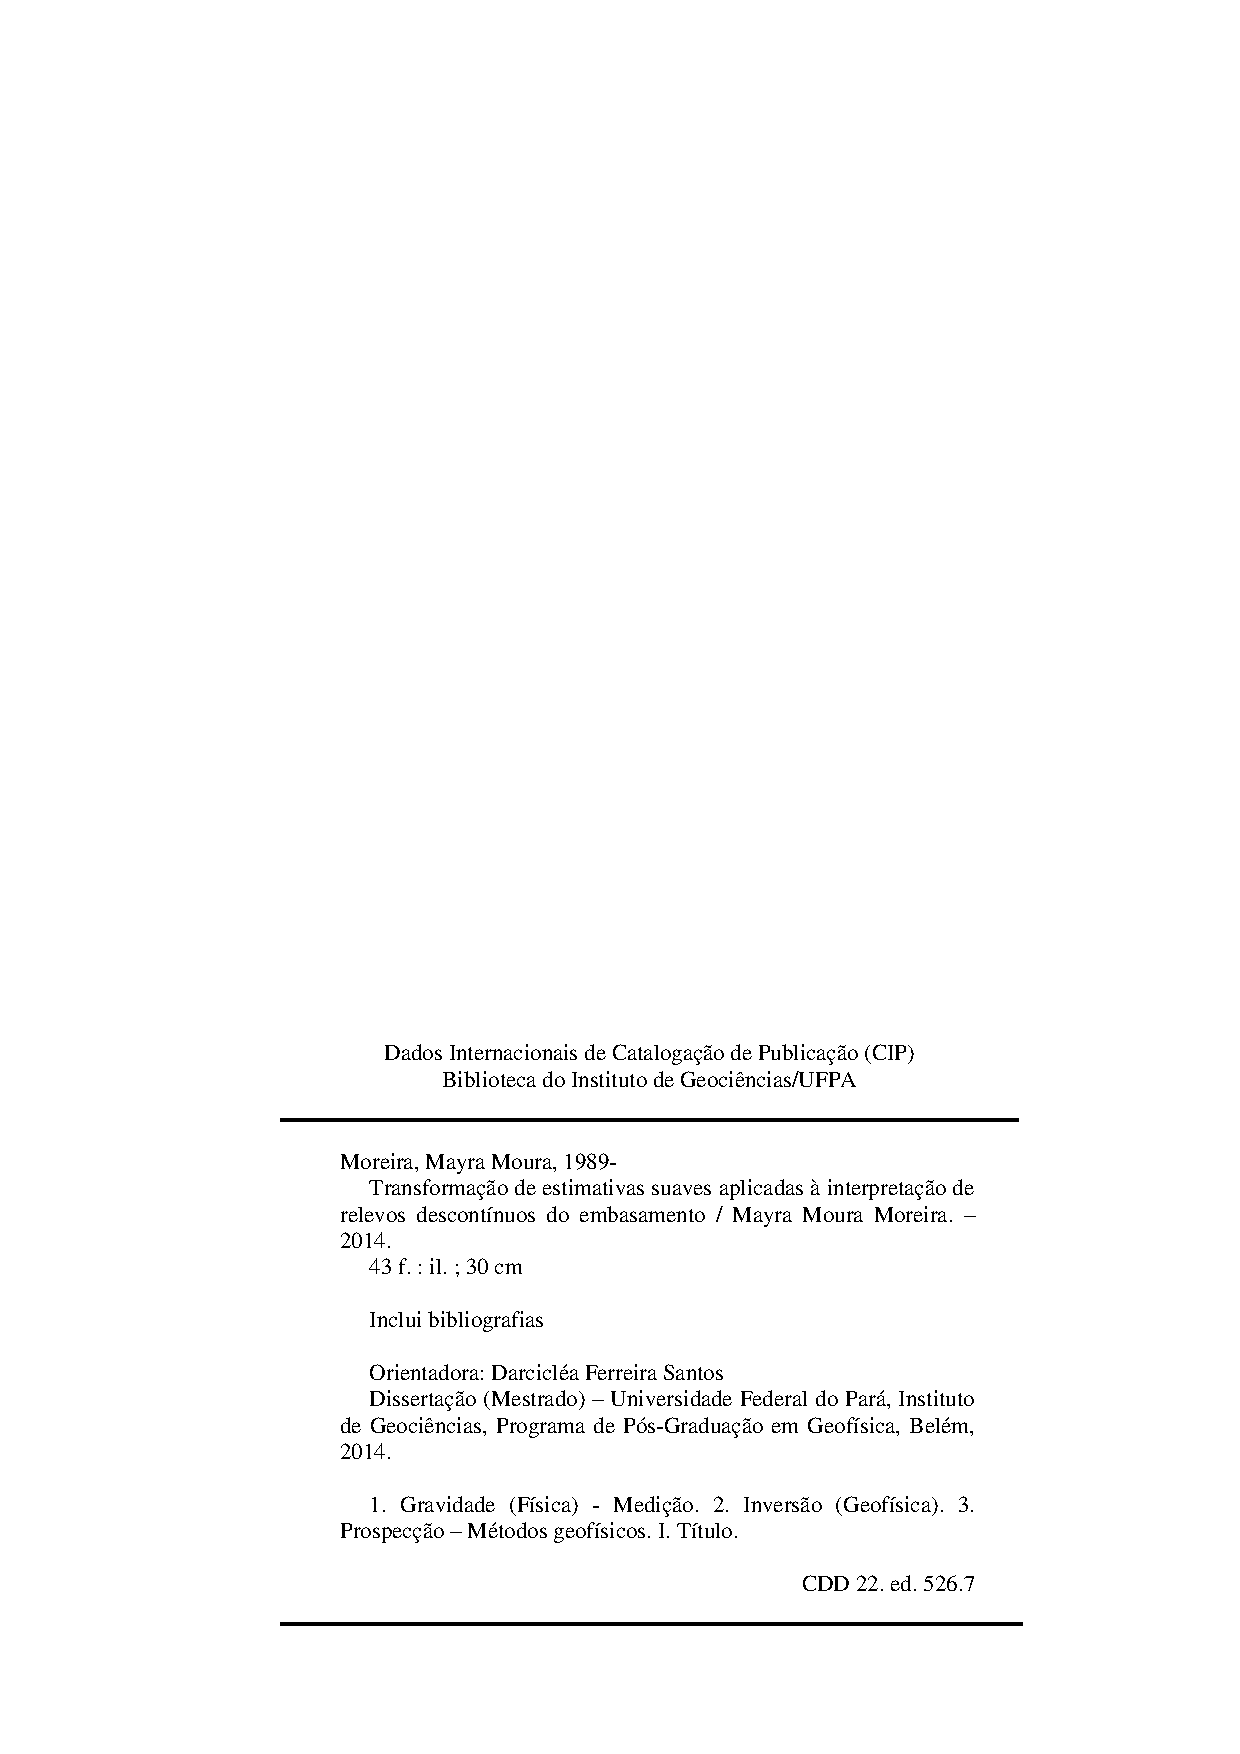
\includepdf[pages=-,pagecommand={},width=\textwidth]{Exemplo_fica_catalografica_2014.pdf}
%% Ficha catalogr\'afica. Comentar comando abaixo quando for imprimir, pois, a 
%% ficha catalogr\'afica deve ser impressa no verso da folha de rosto. 
%% Descomentar ao fazer a vers\~ao eletr\^onica do TCC. Esta ficha deve ser 
%% solicitada através do Sistema FICAT (Sistema de gera\c{c}\~ao de Ficha 
%% Catalogr\'afica da UFPA), dispon\'ivel no site da Biblioteca Central da UFPA, 
%% através do link www.bcficat.ufpa.br/ficha\_catalografica.php. Ela deve estar 
%% no formato pdf.



%\aprovacao{30 de fevereiro de 2020} %%Obrigatorio


%% Este comando \'e Opcional. Caso n\~ao deseje inserir dedicat\'oria, basta 
%% coment\'a-lo. Lembrando que agradecimentos pessoais, relisiosos ou afetivos
%% devem ser feitos aqui. %% Os AGRADECIMENTOS (veja abaixo) devem conter 
%% somente agradecimentos institucionais. 
%\dedicatoria{Ao verme que primeiro roeu as frias carnes do meu cad\'aver\ldots}


%% No arquivo pretextuais.tex dever\~ao ser inclu\'idos: 
%% - AGRADECIMENTOS (obrigat\'orio),
%% - EP\'IGRAFE (opcional),
%% - RESUMO (obrigat\'orio), e
%% - ABSTRACT (obrigat\'orio). 
%% NAO MUDAR O NOME DESTE ARQUIVO.
%%% N\~AO ALTERAR O NOME DESTE ARQUIVO. Neste arquivo s\~ao inseridos os 
%% pr\'e-textos do trabalho.

%%####### AGRADECIMENTOS - obrigat\'orio ##############
\begin{agradecimentos}

Aqui coloco os agradecimentos institucionais. Agradecimentos de car\'ater
pessoais, religiosos ou afetivos devem ser feitos na dedicat\'oria (comando 
presente no arquivo  TEX mestre).
 
\end{agradecimentos}


%%####### EP\'IGRAFE - opcional ##############
%% Caso n\~ao queira incluir ep\'igrafe basta comentar todo o ambiente 
%% abaixo.
\begin{epigrafe}
estamos citando algo.
 
\end{epigrafe}


%%####### RESUMO - obrigat\'orio ################
\begin{resumo}
 isto \'e um resumo.
\end{resumo}

%%####### ABSTRACT - obrigat\'orio ################
\begin{abstract}
 This is an abstract. As you see, it must be written in english.
\end{abstract}

 

%% Listas de figuras, tabelas, siglas, s\'imbolos e abreviaturas: TODAS OPCIONAIS. 

%% Para fazer listas de figuras e de tabelas h\'a comandos espec\'ificos que as 
%% constroem automaticamente. Caso n\~ao queira alguma delas, basta coment\'a-los.
\listoffigures
%\listoftables

%% J\'a as listas de siglas, s\'imbolos e abreviaturas devem ser construidas 
%% pelo autor no arquivo listofsymbols.tex. N\~AO MUDAR O NOME DESTE ARQUIVO.
%\thispagestyle{empty} 
\begin{center} 
\normalfont\bfseries {\large LISTA DE S\'IMBOLOS, SIGLAS E ABREVIATURAS}
\end{center}

%% N\~AO ALTERAR O NOME DESTE ARQUIVO. Neste arquivo s\~ao inseridos as listas 
%% de s\'imbolos, abreviaturas, e ou Siglas usados no trabalho. Adaptar o 
%% t\'itulo e se\c{c}\~oes de acordo com o caso.

\section*{S\'imbolos}

\begin{tabular}{ll}
 $v_P$ & Velocidade da onda P. \\
 $\Delta^{(\mathbf{A})}_{ij}$ & Cofator do elemento $a_{ij}$ da matriz $\mathbf{A}$.
\end{tabular}

\section*{Siglas}

\begin{tabular}{ll}
 EE.UU. & Estados Unidos da Am\'erica. \\
 SBGf & Sociedade Brasileira de Geof\'isica.
\end{tabular}

\section*{Abreviaturas}

\begin{tabular}{ll}
 cont. & continua\c{c}\~ao. \\
 i.e. & isto \'e. \\
\end{tabular}

 

%% SUMARIO - OBRIGATORIO %%%
\tableofcontents        



%%%%%%%%%% - TEXTO - %%%%%%%%%%%%%%%%%%%%
%% cada cap\'itulo deve ter seu arquivo tex. Eles podem ser nomeados livremente
%% bastando que a devida substitui\c{c}\~ao nos comandos abaixo seja feita. Caso
%% queira incluir mais cap\'itulos, basta adicionar mais comandos \include{XXXX}
%% abaixo.

%% Todo cap\'itulo deve come\c{c}\~ao com o comando abaixo o qual deve conter o 
%% t\'itulo do mesmo.
\chapter{Introdução}


Ultimamente, como a industria enfrenta áreas geologicamente mais complexas, os métodos de migração baseados na extrapolação dos campos de onda estão sendo aplicados \citep{claerbout_1971, symes_2008}. Mas, isso se tornou possível, devido às técnicas de aquisição que proporcionam uma melhor iluminação da subsuperfície e os recursos computacionais de alta tecnologia. Esses métodos de imageamento da subsuperfície requer modelos cada vez mais refinados, com isso, uma nova ferramenta de construção de modelos baseada na equação da onda foi estudada, na qual chama-se inversão de onda completa (FWI) \citep{fichtner_2011, virieux_overview_2009, tarantola_2005, tarantola_linearized_1984}. Esse estudo está cada vez mais se tornando um elemento estabelecido do fluxo de processamento sísmicos nos estágios de exploração e monitoramento da produção de óleo e gás por fornecer imagens de alta resolução ajudando, principalmente, na interpretação da subsuperfície estudada. \\

Na inversão sísmica, tem-se como objetivo recuperar o modelo da subsuperfície de modo ``exato''. Mas, a inversão da forma de onda completa (FWI) convencional possui uma complexidade por ser um problema não-linear com muitos minímos locais \citep{bunks_1995}, encontrados na função objetivo e, assim, dificulta-se técnicas de otimização iterativa de trabalhar efetivamente, o qual contribui para uma má recuperação de um bom modelo de velocidade. A presença desses mínimos locais  dificulta a ação dos métodos baseados em gradientes de encontrar uma solução global, deste modo, obtém-se um péssimo modelo de velocidade estimado devido à  má escolha do modelo inicial, o que gera grandes erros entre os dados observados e modelados. No entanto, várias abordagens foram desenvolvidas para reduzir o número de mínimos locais na função objetivo.   \\
 
A inversão completa da onda (FWI) tem como idealização a abordagem da otimização, na qual consiste na mínimização do funcional que realiza o ajuste entre os dados observados e modelados, esse funcional chama-se função objetivo. Mas, para utilizar técnicas de otimização, além da função objetivo, há também  uma necessidade do cálculo do gradiente (direção de máximo crescimento da função objetivo) a partir dos métodos dos estados adjuntos \citep{plessix_2006, fichtner_2011, tarantola_2005}.  
Esses métodos de otimização solucionam problemas para encontrar um valor mínimo ou máximo de uma função não-linear, que podem ser determinísticos ou probabilísticos para encontrar uma melhor solução para o problema proposto. Na literatura, há vários métodos que realizam a minimização, entre os mais utilizados são os métodos do gradiente conjugado (CG), método do gradiente, método de Newton e quase-Newton desenvolvidas nas obras públicadas por \citep{nocedal_2006, nocedal_1980,al-baali_broydens_2013, polak_1965,hestenes_1952,fletcher_1964}. \\

O FWI tem potencial para se tornar a principal ferramenta de construção de modelos da subsuperfı́cie de alta resolução. Porém, é bem conhecido a sua sensibilidade à escolha do modelo inicial, devido à falta de informação de baixo comprimento de onda caracterı́stico dos levantamentos sı́smicos de reflexão. A proposta parte de estudo prévio, no qual é proposto a decomposição dos núcleos de sensibilidade do campo de onda acústico com respeito aos parâmetros do modelo em componentes de fundo e singular. Dessa maneira, as estimativas das perturbações para ambas componentes, de fundo e,principalmente, singular, são pré-determinadas a partir de subnúcleos, de ondas multiplamente espalhadas, de interesse para o cálculo do gradiente, que contém informações de baixa frequência \citep{macedo_2014}. O objetivo desta proposta é combinar os usos, de maneira alternada, dos núcleos de sensibilidade convencional e  dos subnúcleos baseado em espalhamento no processo de inversão, buscando, assim, se beneficiar da autoiluminação complementar propiciada pelos espalhadores existentes no próprio meio.
%Para encontrar uma melhor metodologia para avaliar o gradiente da função objetivo, a fim de definir a direção descendente no processamento de minimização, uma método de decomposição foi criado a partir da decomposição dos núcleos de sensibilidade, esse núcleos são usados para avaliar o gradiente \citep{symes_2008,troltzsch_2010}, e assim, definir uma direção de descida que faça o funcional diminuir \citep{tarantola_2005,fichtner_2011,tarantola_1984}. Então, essa metodologia pressupõem que a decomposição dos núcleos de sensibilidade têm diferentes níveis de iterações entre as componentes do modelo (de fundo e singular) que permite a escolha do mais úteis, dependendo do problema estudado. Essa decomposição foi criada por \citep{macedo_2014} para analisar a interação do campo de onda da componente de fundo e o campo de onda da componente singular em cada parte do núcleo decomposto. Precisamente, essa decomposição foi uma forma de avaliação para encontrar uma melhor direção, consequentemente, um função objetivo apresentando poucos mínimos locais, com isso, linearizando o problema por conta do gradiente desse funcional tenha uma melhor direção de descida para encontrar uma solução global. \\









\section{Objetivo do projeto}
O objetivo central deste projeto é testar a efetividade da decomposição proposta em processo completo de inversão, adicionando as contribuições dos subnúcleos de interesse, logo, aproveitam-se as melhores estimativas da direção para o processo inversão. O caminho mais natural possível é combinar os usos, de maneira alternada, os núcleos de sensibilidade convencional baseados no espalhamento único com os subnúcleos baseados no multiespalhamento proposto por \citet{macedo_2014}, no processo de inversão, busca-se, assim, se beneficiar da autoiluminação complementar propiciada pelos espalhadores existentes no próprio meio. Nesta primeira etapa do projeto planejamos definir um número restrito de modelos 2D
de complexidade estrutural variada, na qual separamos em dois modelos, de fundo obtido a partir da suavização do modelo real e o singular ou perturbação do modelo que será obtido a partir de três estratégias, uma delas é realizar o imageamento utilizando o RTM (``Reverse Time Migration''), outra obtida através da primeira atualização da inversão, que será a estimativa do gradiente ou perturbação do modelo e, por fim, a diferença entre o modelo real com o modelo suavizado. A segunda etapa trata-se de efetivar a utilização da nova metodologia de inversão alternada, com a seleção pré-determinada das contribuições dos subnúcleos obtidas nos resultados do trabalho produzido por \citet{macedo_2014}, em suma, será realizado apenas para poucas atualizações, a fim de realizar testes de acurácia  dos códigos modelados. E por fim, realizar o processo de inversão completa da onda, de modo alternado, para determinar as melhores soluções para os problemas propostos.
%%% Todo cap\'itulo deve come\c{c}\~ao com o comando abaixo o qual deve conter o 
%% t\'itulo do mesmo.
\chapter{Fundamentação teórica}

\section{Problema inverso}
Trata-se de um problema para encontrar a melhor solução para os parâmetros do modelo que descrevem o meio físico \citep{newton_1982}. Para quantificar este problema, é definido um funcional que mostra a diferença entre os dados observados com os dados modelados, se o valor do funcional for mínimo, então os dados modelados estão próximo dos dados observados, logo a estimativa do parâmetro utilizado para obter o dado modelado será solução do problema inverso.
\begin{figure}[htb]
\centering
\includegraphics[width= 9cm, height=6cm]{Figuras/problema_inverso.pdf}
\caption{Problema inverso.} 
\label{fig:problema_inverso}
\end{figure}

Na Figura \ref{fig:problema_inverso} mostra que o problema direto pode ser definido a partir do modelo real, $\mathbf{\text{M}}^{\text{real}}$, podemos encontrar os dados observados, $\mathbf{\text{D}}^{\text{obs}}$. Porém, o problema inverso é definido a partir do modelo estimado,   $\mathbf{\text{M}}^{\text{est}}$, podemos encontrar os dados modelados, $\mathbf{\text{D}}^{\text{mod}}$, se a diferença entre  $\mathbf{\text{D}}^{\text{obs}}$ e $\mathbf{\text{D}}^{\text{mod}}$ for a mínima possível, então teremos uma boa solução do problema. \\

Para resolver esse problema, existe vários métodos de otimização que abrangem abordagens globais e locais que podem ser de maximização ou mínimização de um funcional \citep{nocedal_2006}. Para resolve-lo, precisamos de um método de minimização que irá procurar o valor mínimo do funcional entre os dados observados e modelados, e recursivamente atualizará o modelo estimado até que o funcional esteja no menor valor possível. \\
 
Portanto, para resolver o problema inverso obtendo uma melhor estimativa dos parâmetros, é ter em mãos um método de otimização robusto que tenha uma rápida convergência da minimização do funcional.
\newpage
\section{Métodos de Otimização}

Problemas de otimização podem ser problemas de maximização ou minimização de funções lineares e não-lineares com uma ou mais variáveis em um determinado domínio. Para resolver estes problemas, existem algoritmos que podem ser determinísticos ou probabilísticos. Neste trabalho será apresentado métodos de otimização para solucionar problemas para encontrar o mínimo valor da função objetivo. O esquema de recursão utilizado para resolver esse problema, é dado por
\begin{eqnarray}
\label{xk}
             \mathbf{x}_{k+1} = \mathbf{x}_{k} + \alpha_{k} d_{k} 
\end{eqnarray}
onde $\mathbf{x}$ é o parâmetro da função que irá atualizar iterativamente, $\alpha$ é o comprimento do passo encontrado a partir de alguns métodos de pesquisa de linha e $d_{k}$ é a direção de busca que irá apontar para o mínimo da função, essa direção vai depender do método de otimização utilizado para resolver este problema. A escolha de bons métodos de pesquisa de linha e busca de direção, consequentemente, terá uma boa convergência, e assim, será encontrado mais rapidamente o mínimo da função. \\
 
Para a escolha do tamanho do passo, existem vários métodos de pesquisa de linha presentes na literatura, mas para resolver problemas onde é preciso minimizar funções não-lineares, então é preciso utilizar a abordagem da pesquisa de linha inexata \citep{nocedal_2006}. Essa pesquisa irá aproximar um valor para $\alpha$ que irá depender do método de escolha para um determinada classe de métodos de direção de busca. Usualmente, os métodos da pesquisa de linha são as condições de Wolfe, condição de Armijo, condição de Armijo-Golstein e etc, essas condições permite a avaliação da função objetivo para observar se o tamanho do passo, $\alpha$, está sendo satisfeito para que a função sofra descréscimo. \\

Além disso, há várias classes de métodos para calcular a direção de busca, na qual tem um papel importantíssimo na procura de uma solução otimizada. Dentre eles temos os métodos de Newton, quasi-Newton, Newton-Truncado, Gauss-Newton, gradiente conjugado e etc, que são estão sendo aplicados, cotidianamente, para resolver problemas de otimização. Portanto, para este trabalho, será utilizado dois tipos de métodos de direção de busca, o algoritmo da classe Quasi-Newton e o algoritmo do gradiente conjugado não-linear para resolver o processo de inversão de dados e encontrar uma boa solução para o FWI.   



%\newpage
%\subsection{Busca de linha inexata}
%\subsubsection{Condição de Armijo}
%\newpage
%\subsubsection{Condição de Wolfe}
%\newpage

\subsection{Gradiente conjugado não-linear}
O método originalmente foi projetado e analisado para problemas quadráticos em que a matriz é positiva definida e constante, mas extensões foram realizadas para lidar com problemas não-lineares \citep{polak_1965,hestenes_1952,fletcher_1964}. Esse algoritmo é bastante eficiente, pois, possui um baixo custo computacional, visto que necesssita apenas do gradiente do funcional, o que torna-o bastante efetivo para solucionar problemas em grande escala. Portanto, dada uma aproximação inicial, $\mathbf{x}_{0} \in \mathbb{R}^{n}$, aplicando a busca de linha inexata, então teremos um conjunto de direções conjugadas para $k$ iterações, a direção de busca é definida por % A abordagem nesse trabalho é a aplicação do gradiente conjugado não-linear com descida garantida \citep{hager_2005} aplicado para três diferentes parâmetros $\beta_{k}$  \citep{polak_1965,hestenes_1952,fletcher_1964} para resolver um problema de otimização sem vínculo. Esse método obedece a recorrência da equação \ref{xk}, então o cálculo da direção de busca é definido por
    \begin{eqnarray}
         \label{dirdesc}
            d_{k}  = \left\{ \begin{array}{rll}
           {d(0)= -g(0)} ~~~~~~~~~~~~~~~ &{, k=0} \\
           {d_{k+1} =-g_{k+1}+\beta_{k} d_{k} ~~~~~}   
          \end{array} \right.
          \end{eqnarray}
onde $g$ é o gradiente , $k$ é a iteração e $\beta_{k}$ são os parâmetros que diferenciam a direção de busca, esses parâmetros possui um risco crítico no gradiente, pois afeta a taxa de convergência para a solução do problema  e eles são definidos por :
\begin{eqnarray}
          \nonumber
          \beta_{HS} = \frac{g_{k}^{T}~y_{k-1}}{d^{T}_{k-1} y_{k-1}}, ~~~ \beta_{PRP} = \frac{g_{k}^{T} y_{k-1}}{\left\|g_{k-1}\right\|^{2}}, ~~~\beta_{LS} = \frac{g_{k}^{T} y_{k-1}}{-d_{k-1}^{T} g_{k-1} } \\ \nonumber
          \\ \nonumber \\ \nonumber
          \beta_{DY} = \frac{\left \| g_{k} \right \|^{2}}{d^{T}_{k-1} y_{k-1}}, ~~~\beta_{FR} = \frac{\left \| g_{k}\right \|^{2}}{\left \| g_{k-1}\right \|^{2}},~~~ \beta_{CD} = \frac{\left \| g_{k}\right \|^{2}}{-d_{k-1}^{T} g_{k-1} }
          \end{eqnarray}
onde
\begin{eqnarray}
 \nonumber
y_{k} = g_{k+1} - g_{k}
\end{eqnarray}

onde $y_{k}$ é uma equação auxiliar. Observa-se na equação \ref{dirdesc} que para encontrar a direção de descida,$d_{k}$, é necessário realizar uma recursão, na qual é essencial para cada atualização, o cálculo do gradiente a partir da solução encontrada com a melhor direção de descida, o que faz o funcional convergir e obter uma melhor solução possível para resolver o    problema. Entretanto, para o método de gradiente conjugado, os vários parâmetros $\beta$ encontrados na literatura, influenciam fortemente para a resolução do problema, visto que esses parâmetros dão um peso para a próxima direção de descida que irá ser calculado, como é observado na equação \ref{dirdesc}. 

Portanto, a escolha dos parâmetros serão importantes para resolver o problema com êxito. Dessa maneira, escolher os parâmetros que possuem os cálculos de convergência serão optados para ter uma boa convergência do método, pois tem-se uma segurança a mais para resolver problemas em grande escala. Destarte, o método possui uma grande facilidade de implementação e, como informado acima, possui um baixo custo computacional. 

\newpage
\subsection{LBFGS-B Quasi-Newton}
Todo problema de otimização é necessário minimizar uma função não linear,$f(\matbf{x})$, para obter uma melhor solução possível,$\mathbf{x}$, principalmente, quando temos o gradiente disponível, então, para solucionar esse problema, utilizaremos uma classe de métodos de otimização chamada Quasi-Newton. Esse método é baseado na projeção do gradiente, onde aproxima a matriz Hessiana a partir da matriz Jacobiana inversa \citep{byrd_representations_1994,al-baali_broydens_2013}. A partir dessa aproximação, usaremos o algoritmo LBFGS-B formulado por \citet{zhu_algorithm_1997}, na qual é desenvolvido a partir da aproximação da matriz Hessiana utilizando a matriz BFGS de memória limitada criado por \citet{nocedal_1980}. \\

 No entanto, quando há problemas de grande porte, as técnicas de atualização do método Quasi-Newton tornam-se caras computacionalmente, pois a aproximação da Hessiana ocupa um grande espaço. Porém, o diferencial desse algoritmo é uma adaptação da matriz BFGS que consiste na otimização de memória onde as informações antigas da matriz são descartadas e substituidas pelas novas atualizações, com isso, facilitando a construção da matriz de aproximação da Hessiana sem ocupar um grande volume de dados \citep{morales_remark_2011,zhu_algorithm_1997}, o que torna o método um ótimo método de minimização para solução de problemas. \\
 
 

%O algoritmo LBFGS-B propõem minimizar uma função não linear com $n$ variáveis sujeitos aos limites, $l\le \mathbf{x}\le u$, na qual são os vetores dos limites inferiores e superiores, respectivamente. 







\newpage
\section{Método dos Estados Adjuntos}
O método dos estados adjuntos é uma metologia para calcular o gradiente de um certo funcional em relação aos parâmetros que envolvem essa função \citep{fichtner_full_2011,virieux_overview_2009}. Se tratando de inversão, é desejado encontrar os parâmetros que melhor descrevem os dados observados, mas para encontrar esses parâmetros ótimos irá depender das técnicas de otimização \citep{nocedal_2006}. Como foi visto acima, todas as técnicas de otimização requer o cálculo do gradiente da função objetivo em relação aos parâmetros do modelo para atualizar a cada iteração o modelo de velocidade que melhor se adequa ao modelo verdadeiro. \\

 No entanto, no método, a função objetivo depende dos parâmetros do modelo através das variáveis de estado \citep{plessix_2006}. Dessa maneira, significa que o gradiente da função objetivo depende do gradiente do campo de onda em relação aos parâmetros do modelo \citep{fichtner_2011}.  Esse método matemático é uma ferramenta capaz que permite calcular o gradiente de um funcional sem da necessidade de construir a matriz sensibilidade. De uma maneira geral, será possível definir um problema de otimização com a minimização de uma função objetivo, então, temos que 

\begin{eqnarray}
\label{objfunction}
 \mathcal{F}(\mathbf{m}) = \frac{1}{2} \left \| \mathbf{u}(\mathbf{m}) - d^{obs} \right \|^{2},
\end{eqnarray}
\begin{eqnarray}
 \label{equacaoestado}
 F(\mathbf{u}(\mathbf{m}), \mathbf{m} ) = 0,
\end{eqnarray}

onde $\mathbf{m}$ corresponde aos parâmetros do modelo, $\mathbf{u}(\mathbf{m})$ corresponde a váriável de estado que satisfaz a equação de estado \ref{equacaoestado} e $d^{obs}$ está relacionado aos dados observados. Para calcular o gradiente da função objetivo \ref{objfunction}, é preciso definir a Lagrangeana $\mathcal{L}$ , então

\begin{eqnarray}
\label{lagrange123}
 \mathcal{L} (\mathbf{u}, \mathbf{m}, \Lambda) = \mathcal{F}(\mathbf{u},\mathbf{m}) + \langle F(\mathbf{u}, \mathbf{m}), \Lambda\rangle ,
\end{eqnarray}

onde $\Lambda$ é a varíavel de estado adjunto que não depende dos parâmetros do modelo. Como a equação de estado \ref{equacaoestado} é zero para qualquer $\Lambda$ e a mesma não depende dos parâmetros do modelo, então

\begin{eqnarray}
  \frac{\partial \mathcal{F}}{\partial \mathbf{m}} = \frac{\partial \mathcal{L}}{\partial \mathbf{m}}
\end{eqnarray}


A partir disso, é possível determinar o gradiente da função objetivo $\mathcal{F}$ avaliando a variação de primeira ordem da Lagrangeana em relação a uma configuração estácionaria. Agora será realizado a perturbação dos parâmetros do modelo $\delta \mathbf{m}$ e da variável de estado $\delta \mathbf{u}$, através de uma aproximação de primeira ordem para $\Lambda$ fixo, então

\begin{eqnarray}
\label{lagrange12}
 \delta \mathcal{L} = \frac{\partial \mathcal{L}}{\partial \mathbf{u}} \delta \mathbf{u} + \frac{\partial \mathcal{L}}{\partial \mathbf{m}} \delta \mathbf{m}
\end{eqnarray}


Realizando o cálculos da equação \ref{lagrange12} e exigindo que a variação da função objetivo ocorra devido a variação dos parâmetros do modelo, é possível obter a equação adjunta e a fonte adjunta. A partir das equações descritas acima, é possível a aplicação do método adjunto nas equações acústicas da onda que é definida por
\begin{eqnarray}
 \frac{1}{c^{2}(\mathbf{x})} \frac{\partial ^{2} p(\mathbf{x},t)}{\partial t^{2}} - \nabla^{2} p(\mathbf{x},t) = f(\mathbf{x},t)
\end{eqnarray}

pnde $p(\mathbf{x},t)$ é o campo de pressão, $c(\mathbf{x})$ é o modelo de velocidade, $\mathbf{x}$ é o vetor posição e $f(\mathbf{x},t)$ é o termo fonte. A equação de estado para esse problema é dado por 
\begin{eqnarray}
\label{f_esta}
 F(p,c) = \frac{1}{c^{2}(\mathbf{x})} \frac{\partial ^{2} p(\mathbf{x},t)}{\partial t^{2}} - \nabla^{2} p(\mathbf{x},t) - f(\mathbf{x},t) = 0
\end{eqnarray}


A função objetivo é expressa por 
\begin{eqnarray}
  \mathcal{F} = \frac{1}{2} \sum_{s} \sum_{r} \int_{0}^{T} \left[ p^{obs} (t,\mathbf{x}_{r};\mathbf{x}_{s}) - p^{mod}(t,\mathbf{x}_{r};\mathbf{x}_{s};c(\mathbf{x})) \right ] ^{2} dt
  \label{func_obj}
\end{eqnarray}

onde $\mathbf{x}_{r}$ e $\mathbf{x}_{s}$ são as posições do receptor e da fonte, respectivamente, $p^{obs}$ corresponde ao campo observado e $p^{mod}$ corresponde ao campo modelado. O problema de otimização consiste em minimizar a função objetivo $\mathcal{F}$ juntamente com a equação de estado. Com isso, pode-se definir a lagrangeana para o problema, então substituindo a equação \ref{f_esta} e \ref{func_obj}  em \ref{lagrange123}, temos

\begin{eqnarray}
\mathcal{L}(c, p, \Lambda)=\frac{1}{2} \sum_{s} \sum_{r} \int_{0}^{T}\left[p^{o b s}\left(t, \mathbf{x}_{\mathbf{r}} ; \mathbf{x}_{\mathbf{s}}\right)-p^{mod}\left(t, \mathbf{x}_{\mathbf{r}} ; \mathbf{x}_{\mathbf{s}} ; c(\mathbf{x})\right)\right]^{2} d t 
\end{eqnarray}
\begin{eqnarray}
\nonumber
&+\sum_{s} \int_{\Omega} d \Omega \int_{0}^{T} d t \Lambda(t, \mathbf{x})\left[\frac{1}{c^{2}(\mathbf{x})} \frac{\partial^{2} p(t, \mathbf{x})}{\partial t^{2}}-\nabla^{2} p(t, \mathbf{x})-f(\mathbf{x},t)\right]
\end{eqnarray}

onde $\Lambda(t,\mathbf{x})$ é a varíavel adjunta que não depende dos parâmetros do modelo. O gradiente do funcional $\mathcal{F}$ pode ser avaliado a partir da variação de primeira ordem da Lagrangeana em relação a perturbação do modelo de velocidade, na qual, induz uma perturbação no campo de pressão. Com isso, a variação da Lagrangeana é dada por 
\begin{eqnarray}
 \delta \mathcal{L} = \frac{\partial \mathcal{L}}{\partial c} \delta c + \frac{\partial \mathcal{L}}{\partial p} \delta p
\end{eqnarray}

calculando as derivadas parciais e realizando cálculos e substituições posteriores, é possível definir a variação do funcional em relação aos parâmetros do modelo, o que permite obter a equação para o campo adjunto, onde é expresso por 
\begin{eqnarray}
 \frac{1}{c^{2}(\mathbf{x})} \frac{\partial^{2} \Lambda(t, \mathbf{x})}{\partial t^{2}}-\nabla^{2} \Lambda(t, \mathbf{x})=\left[p^{o b s}\left(t, \mathbf{x} ; \mathbf{x}_{\mathbf{s}}\right)-p^{mod}\left(t, \mathbf{x} ; \mathbf{x}_{\mathbf{s}}\right)\right] \delta\left(\mathbf{x}-\mathbf{x}_{r}\right)
 \label{campoadjunto}
\end{eqnarray}

onde o resíduo do campo de pressão observado e modelado é a fonte adjunta. Essa equação está sujeita a certas condições, então 
\begin{eqnarray}
\left.\Lambda\left(T, \mathbf{x} ; \mathbf{x}_{s}\right)\right|_{\Omega} &=0 \\ \nonumber
\left.\frac{\partial \Lambda\left(T, \mathbf{x} ; \mathbf{x}_{s}\right)}{\partial t}\right|_{\Omega} &=0
\end{eqnarray}

e as condições de fronteira homogêneas
\begin{eqnarray}
 \Lambda (t, \mathbf{x}; \mathbf{x}_{s} |_{\partial \Omega} = \nabla \Lambda (t,\mathbf{x};\mathbf{x}_{s}) |_{\partial \Omega} = 0
\end{eqnarray}

O gradiente da função objetivo pode ser observado pela parcela não nula da variação da Lagrangeana 
\begin{eqnarray}
 \delta \mathcal{L}=\int_{\Omega} d \Omega \delta c(\mathbf{x}) \frac{\partial \mathcal{F}}{\partial c(\mathbf{x})}
\end{eqnarray}

onde o gradiente do funcional $\mathcal{F}$ é dado por 
\begin{eqnarray}
 \frac{\partial \mathcal{F}}{\partial c(\mathbf{x})} \equiv-\frac{2}{c^{3}(\mathbf{x})} \sum_{s} \int_{0}^{T} d t \Lambda\left(t, \mathbf{x} ; \mathbf{x}_{\mathbf{s}}\right) \frac{\partial^{2} p\left(t, \mathbf{x} ; \mathbf{x}_{\mathbf{s}}\right)}{\partial t^{2}}
\end{eqnarray}


  onde $\Lambda\left(t, \mathbf{x} ; \mathbf{x}_{\mathbf{s}}\right)$ é o campo adjunto retropropagado pelo resíduo dos campos de pressão observado e modelado, $p$ é o campo da modelagem direta.
\newpage
\section{Aproximação de Born}
A aproximação de Born de primeira ordem é uma aproximação de espalhamento único, usada nas aplicações sísmicas para aproximar o campo de onda pertubado devido a pertubação no meio de referência \citep{tarantola_2005, keys_1983}. Essa metodologia é uma forma de linearizar o campo de onda no problema direto para obter uma solução aproximada do campo de origem. Problemas relacionados com a equação da onda, onde a solução conhecida corresponde ao comportamento não linear entre equação da onda e o parâmetro do modelo, utilizando a metodologia, a solução será linearizada, e assim, transformando uma problema não linear em um problema linear. A equação da onda é dada por

\begin{eqnarray}
\frac{1}{c^{2}(\mathbf{x})} \frac{\partial^{2} p(\mathbf{x},t) }{\partial t^{2}} - \nabla^{2} p(\mathbf{x},t) = f(\mathbf{x},t)
\label{eq_wavefield}
\end{eqnarray}

onde $c$ é a velocidade, $p$ é o campo de pressão, $\mathbf{x}$ é a posição e $f(\mathbf{x},t)$ é o termo fonte, e usualmente, é definido por $f(\mathbf{x},t) = \delta (\mathbf{x}-\mathbf{x}_{s})~S(t)$, onde o termo $\delta (\mathbf{x}-\mathbf{x}_{s})$ é a localização da fonte e $S(t)$ é a wavelet mostrando a história da fonte. Aplicando a teoria da pertubação no modelo de velocidade, e consequentemente, no campo de onda, temos que
\begin{eqnarray}
 c(\mathbf{x}) = c_{0}(\mathbf{x}) + \delta c(\mathbf{x}) ~~~~~~~~~ p(\mathbf{x},t) = p_{0}(\mathbf{x},t) + \delta p(\mathbf{x},t)
 \label{eq_perturbation}
\end{eqnarray}
onde $c_{0}(\mathbf{x})$ é a velocidade de referência, $\delta c(\mathbf{x})$ é a velocidade perturbada, $p_{0}(\mathbf{x},t)$ é o campo de onda de referência e $\delta p(\mathbf{x},t)$ é o campo de onda perturbado.
Realizando a substituição da equação \ref{eq_perturbation} em \ref{eq_wavefield}, temos

\begin{eqnarray}
 \frac{1}{\left[c_{0}(\mathbf{x})+\delta c(\mathbf{x})\right]^{2}} \frac{\partial^{2} \left[p_{0}(\mathbf{x},t) + \delta p(\mathbf{x},t) \right]}{\partial t^{2}} - \nabla^{2} \left[p_{0}(\mathbf{x},t)+ \delta p(\mathbf{x},t) \right] = f(\mathbf{x},t)
 \label{eq_wavefield_perturbation}
\end{eqnarray}

A partir da equação acima, será realizada a aproximação de primeira ordem do primeiro termo da equação, então
\begin{eqnarray}
 \frac{1}{\left[c_{0}(\mathbf{x})+\delta c(\mathbf{x})\right]^{2}} \approx \left[ \frac{1}{c_{0}(\mathbf{x})^{2}} - \frac{2~\delta c(\mathbf{x})}{c_{0}^{3}(\mathbf{x})} \right ]
 \label{approximation_first_order}
\end{eqnarray}

Substituindo a equação \ref{approximation_first_order} em \ref{eq_wavefield_perturbation}, temos que
\begin{eqnarray}
 \left[ \frac{1}{c_{0}(\mathbf{x})^{2}} - \frac{2~\delta c(\mathbf{x})}{c_{0}^{3}(\mathbf{x})} \right ]
\frac{\partial^{2} \left[p_{0}(\mathbf{x},t) + \delta p(\mathbf{x},t) \right]}{\partial t^{2}} - \nabla^{2} \left[p_{0}(\mathbf{x},t)+ \delta p(\mathbf{x},t) \right] = f(\mathbf{x},t)
\end{eqnarray}

Realizando as distribuições e substituições, é encontrado o campo de onda perturbado, então
\begin{eqnarray}
 \frac{1}{c_{0}^{2}(\mathbf{x})} \frac{\partial^{2} \delta p(\mathbf{x},t)}{\partial t^{2}} - \nabla ^{2} \delta p(\mathbf{x},t) = \left [\frac{2\delta c(\mathbf{x})}{c_{0}^{3}(\mathbf{x})} \right ] \frac{\partial^{2} p_{0}(\mathbf{x},t)}{\partial t^{2}}
 \label{eq_perturbation_linearized}
\end{eqnarray}

onde o termo fonte depende do campo de onda de referência. A equação \ref{eq_perturbation_linearized} corresponde à forma linearizada da equação da onda perturbada utilizando a aproximação de born como descrito por \citet{keys_1983}. Em outras palavras, temos a aproximação da relação linear entre o campo onda perturbado $\delta p$ e o modelo de velocidade perturbado $\delta c$. Para realizar a modelagem do campo de onda perturbado, será preciso modelar o campo de onda utilizando o modelo de velocidade de referência, pois o termo fonte da equação \ref{eq_wavefield_perturbation}  é dependente desse campo de onda. Realizando essa aproximação, a modelagem irá considerar apenas reflexões primárias no campo de onda. A Figura \ref{approximation_born} mostra o comportamento da aproximação de acordo com o que foi descrito acima.
\begin{figure}[htb]
\centering
\includegraphics[width=12cm, height=8cm]{Figuras/approximation_born.pdf}
\caption{Sistema do problema de espalhamento do campo de onda, onde o meio foi decomposto em duas partes : meio de fundo $c_{0}$ e o meio perturbado ou espalhado  $\delta c$, e os campos correspondentes, $p_0$ campo de onda de referência e $\delta p$ campo de onda perturbado.}
\label{approximation_born}
\end{figure}







\newpage
\section{Migração reversa no tempo}

Há muitos métodos de migração de dados sísmicos, mas um dos métodos mais preciosos é a migração reversa no tempo. A metodologia é capaz de lidar com diversas variações de velocidade, de modo que torna o método atrativo para o imageamento de estruturas complexas \citep{baysal_1983}. Entretanto, o intuito físico é que os campos de onda devem correlacionar nas iterfaces refletoras através dos campos de onda da fonte e dos receptores, essa métodologia é denominada de condição de imagem. \\

A condição de imagem tem como objetivo formar uma imagem ponto a ponto em cada intervalo temporal para gerar uma imagem migrada a partir de uma correlação cruzada entre os campos (fonte e receptor). Matematicamente, esse método correlaciona os campos de fonte com os campos de receptores no espaço e no tempo, então temos:

\begin{eqnarray}
 I (\mathbf{z},\mathbf{x}) = \int_{0}^{t} dt~~~ p_{f}(\mathbf{z},\mathbf{x};t)~*~ p_{r}(\mathbf{z},\mathbf{x};t)
 \label{eq:correlation_rtm}
\end{eqnarray}
\\
onde $I$ é a imagem migrada, $p_{f}$ é o campo de onda gerada pela fonte e $p_{r}$ é o campo de onda gerado pelo receptor. O campo de onda gerada pela fonte, $p_{f}$, é gerado a partir de uma aquisição sísmica utilizando um modelo de velocidade pré-determinado observado na Figura \ref{fig:rtm}, esse sinal recebido pelo receptor irá se tornar a fonte para gerar o campo de onda dos receptores,$p_{r}$, observado na Figura \ref{fig:rtm_2} e, assim, se propagar para correlacionar ponto a ponto para gerar a imagem.

\begin{figure}[h!]
\centering
\subfigure[Campo de onda da fonte]{
    \includegraphics[width=0.40\textwidth]{Figuras/rtm.pdf}
    \label{fig:rtm}}
  \subfigure[Campo de onda dos receptores]{
    \includegraphics[width=0.40\textwidth]{Figuras/rtm_2.pdf}
    \label{fig:rtm_2}}
   
  \caption{As Figuras mostram os processos realizados para realizar a migração reversa no tempo: (a) é o processo que gera o campo de onda da fonte que evolui para frente no tempo e (b) mostra o processo que gera o campo de onda dos receptores que evolui para trás no tempo. }
\end{figure}

 Destarte, obtêm-se os dois campos de onda (``forward'' e ``backward''), logo, é necessário aplicar a condição de imagem (correlação cruzada) da equação \ref{eq:correlation_rtm} para extrair a imagem migrada da subsuperfície estudada. Portanto, o método RTM (``Reverse time migration'' ou Migração reversa no tempo) é uma ótima ferramenta de imageamento da subsuperfície, além de ter excelentes resultados para modelos de velocidade com variações laterais. Na literatura, há muitas maneiras de aplicação desse método para obter um melhor imageamento da subsuperfície, como, por exemplo, uma aplicação é a aproximação de born, na qual essa metodologia faz com que os campos de onda tenha apenas reflexões primárias, destarte, eliminando múltiplas e outros dados não-essenciais.

\chapter{Fundamentos Teóricos}


\section{Migração reversa no tempo}

Há muitos métodos de migração de dados sísmicos, mas um dos métodos mais preciosos é a migração reversa no tempo. A metodologia é capaz de lidar com diversas variações de velocidade, de modo que torna-se o método atrativo para o imageamento de estruturas complexas \citep{baysal_1983}. Entretanto, o intuito físico é que os campos de onda devem correlacionar nas iterfacies refletoras, através dos campos de onda da fonte e dos receptores, essa métodologia é denominada de condição de imagem. 

A condição de imagem tem como objetivo formar uma imagem, ponto a ponto, em cada intervalo temporal, para gerar uma imagem migrada a partir de uma correlação cruzada entre os campos (fonte e receptor). Matematicamente, esse método correlaciona os campos da fonte com os campos dos receptores no espaço e no tempo, então temos:

\begin{eqnarray}
 I (\mathbf{z},\mathbf{x}) = \int_{0}^{t} dt~~~ p_{f}(\mathbf{z},\mathbf{x};t)~*~ p_{r}(\mathbf{z},\mathbf{x};t)
 \label{eq:correlation_rtm}
\end{eqnarray}
onde $I$ é a imagem migrada, $p_{f}$ é o campo de onda gerada pela fonte e $p_{r}$ é o campo de onda gerado pelo receptor. O campo de onda gerada pela fonte, $p_{f}$, é gerado a partir de uma aquisição sísmica utilizando um modelo de velocidade pré-determinado observado na Figura \ref{fig:rtm}, esse sinal recebido pelo receptor irá se tornar a fonte para gerar o campo de onda dos receptores,$p_{r}$, observado na Figura \ref{fig:rtm_2} e, assim, se propagar para correlacionar, ponto a ponto , para gerar a imagem.

\begin{figure}[h!]
\centering
\subfigure[Campo de onda da fonte]{
    \includegraphics[width=0.40\textwidth]{Figuras/rtm.pdf}
    \label{fig:rtm}}
  \subfigure[Campo de onda dos receptores]{
    \includegraphics[width=0.40\textwidth]{Figuras/rtm_2.pdf}
    \label{fig:rtm_2}}
   
  \caption{As Figuras mostram os processos realizados para realizar a migração reversa no tempo: (a) é o processo que gera o campo de onda da fonte que evolui para frente no tempo e (b) mostra o processo que gera o campo de onda dos receptores que evolui para trás no tempo. Fonte : Autor }
\end{figure}

 Destarte, obtêm-se os dois campos de onda (``forward'' e ``backward''), logo, é necessário aplicar a condição de imagem (correlação cruzada) da equação \ref{eq:correlation_rtm} para extrair a imagem migrada da subsuperfície estudada. Portanto, o método RTM (``Reverse time migration'' ou Migração reversa no tempo) é uma ótima ferramenta de imageamento da subsuperfície e ainda possui excelentes resultados para modelos de velocidade com variações laterais. No entanto, na literatura, existem muitas maneiras de aplicação desse método para obter um melhor imageamento da subsuperfície, como, por exemplo, uma aplicação é a aproximação de born, na qual essa metodologia faz com que os campos de onda tenha apenas reflexões primárias, dessarte, elimina-se múltiplas e outros dados não-essenciais.

%Com base na função objetivo, na qual é o desajuste entre os dados observados e modelados, precisamos determinar um modelo inicial, $m_{0}$, para obter os dados modelados. Possuindo os dados observado, $d^{obs}$, o modelo inicial, $m_{0}$, e os dados observado 
\section{FWI baseado na decomposição dos núcleos de sensibilidade}
O intuito desse capítulo é descrever o papel da decomposição desses núcleos iterativos do FWI a partir da metodologia criada por \citet{macedo_2014}, na qual utiliza a abordagem da teoria do espalhamento para decompor os núcleos de sensibilidade \citep{tarantola_linearized_1984}. Essa decomposição é realizada para encontrar informações sobre o  modelo de fundo a partir de um campo multiplamente espalhado, pois elas se propagam através do meio por tempo longo o bastante a ponto de carregar esse tipo de informação \citep{snieder_2002}. 

Ademais, se tratando de inversão não-linear convencional baseado em gradientes, a escolha de um modelo inicial será limitada e causará uma insensibilidade no comprimento de onda longo \citep{gauthier_1986,mora_1987,claerbout_1976,jannane_1989} e, assim, causando a existência de vários mínimos locais na função objetivo \citep{bunks_1995}, com isso, esses mínimos locais impedem que encontrem o mínimo global quando o modelo inicial está longe da solução global. Nos trabalhos de \citet{jannane_1989} e \citet{claerbout_1976} mostram que as baixas frequências são sensíveis quando o modelo de fundo é perturbardo e as altas frequências são sensíveis as perturbações do modelo de refletividade. Portanto, para contornar o problema de minímos locais,será  realizado a decomposição proposta, o que reparametriza o meio de referência em duas partes (fundo e singular), assim, gerando dois campos, um campo de onda de fundo sensível apenas ao modelo de fundo e um campo de onda singular sensível as duas partes do modelo e, também, dois resíduos dos campos de onda (fundo e singular) para aplicar a redecomposição para calcular os gradientes. 


\section{Inversão de onda completa}

A inversão de onda completa (FWI) baseia-se na minimização de uma função objetivo que utiliza métodos de otimização para encontrar uma solução ótima que melhor descreva os dados observados. Os dados observados, $d^{obs}$, é obtido a partir de um modelo de parâmetros real, $\mathbf{m}$, que descreve a subsuperfície. Matemáticamente, para obter o campo de excitação resultante, é necessário determinar o problema direto \citep{menke_1989}:

\begin{eqnarray}
\mathbf{d} = \mathbf{L}(\mathbf{m}),
\label{eq:campo_direto}
\end{eqnarray}
\\
onde $\mathbf{L}$ é o operador físico-matemático entre o campo de onda e o modelo. Na inversão convencional esse problema seria resolvido analiticamente encontrando o operador $\mathbf{L}^{-1}$, de modo que os parâmetros do modelo, $\mathbf{m}$, seria encontrado a partir do campo de excitação, $\mathbf{d}$, pela relação $\mathbf{m} = \mathbf{L}^{-1}(\mathbf{d})$. Contudo, na inversão de dados sísmicos, o problema de inversão é altamente não-linear e, com isso,  dificulta obter analiticamente o operador $\mathbf{L}^{-1}$. \\

Além disso, se tratando no contexto de exploração sísmica, o campo obtido ao longo do tempo a partir de um modelo que representa a subsuperfície, denominamos de dado observado, $\mathbf{d}^{obs}$. Geralmente, temos informações a piori  que representaria as informações iniciais dos parâmetros do modelo, denominamos essas informações iniciais como modelo inicial, $\mathbf{m}_{0}$. Realizando a modelagem do campo, ao longo do tempo, a partir da equação \ref{eq:campo_direto} utilizamos o modelo inicial, $\mathbf{m}_{0}$, teremos os dados modelados, $\mathbf{d}^{mod}$. Com esses dados, podemos construir o problema do FWI, na qual consiste em encontrar uma estimativa do melhor modelo de velocidade a partir de sucessivas iterações, então podemos definir a função objetivo como:

\begin{eqnarray}
       \mathcal{F} = \left \| \mathbf{d}^{mod} - \mathbf{d}^{obs} \right \| ^{2}_{2} 
\end{eqnarray}
\\

onde $\|.\|_{2}$ é a forma da norma ${l}_{2}$. A partir da definição da função objetivo, o FWI tem como objetivo principal minimizar a função objetivo para obter uma melhor estimativa do modelo de velocidade.
\section{Núcleo de sensibilidade}


Neste trabalho será abordado a equação da onda acústica, onde descreve a evolução do campo de onda através de um meio caracterizado por um ou dois parâmetros. Consideramos uma fonte pontual e adicionando condições iniciais, a equação da onda é definida por\\
\begin{eqnarray}
\frac{1}{c^{2}(\mathbf{x})} \frac{\partial^{2} p(\mathbf{x},t)}{\partial t^{2}} - \nabla^{2}p(\mathbf{x},t) = \delta(\mathbf{x}-\mathbf{x}_{s}) S(t) 
\label{eq_wave}
\end{eqnarray}
\\
onde $\mathbf{x}_{s}$ indica a posição da fonte e $S(t)$ a história da fonte (wavelet). Por questão de simplicidade e simplificação, iremos considerar um operador do campo de onda $\mathcal{L}$ que é definido por \\
\begin{eqnarray}
     \mathcal{L} = \frac{1}{c^{2}(\mathbf{x})} \frac{\partial^{2} }{\partial t^{2}} - \nabla^{2}
     \label{operador_wave}
\end{eqnarray}
\\
onde $c(\mathbf{x})$ é a velocidade que descreve o meio e está presente no vetor parâmetro $\mathbf{m}$. Realizamos a substituição da equação \ref{operador_wave} em \ref{eq_wave}, então \\

\begin{eqnarray}
      \mathcal{L}\left[p(\mathbf{x},t;\mathbf{x}_{s})\right] = \delta(\mathbf{x}-\mathbf{x}_{s}) S(t)
      \label{l_wave}
\end{eqnarray}
\\
onde é uma representação da forma reduzida da equação \ref{eq_wave} que usaremos na descrição teórica. A solução da equação da onda apresenta uma relação não-linear entre o funcional e vetor de parâmetros que pode ser representados por \\
\begin{eqnarray}
 p = f (\mathbf{m})
 \label{funcional_p}
\end{eqnarray}
\\
onde $f$ é o funcional relacionado ao campo de onda $p$ e o vetor parâmetro $m$. Esse funcional irá depender do método utilizado para a problema direto e do modelo de velocidade. \\


%\subsection{Teoria do espalhamento}
%\textbf{Falar um pouco da teoria} \\
Outrossim, utilizamos a teoria clássica do espalhamento, visto que o campo total $p$ se propaga em um modelo de velocidade que descreve o meio, na qual é decomposto em duas componentes : um campo de onda de referência, $p_{0}$, e um campo de onda disperso, $p_{S}$, de modo que, a soma das duas componentes teremos o campo total ($p = p_{0} + p_{s}$). O campo de onda de referência é gerado pela fonte original referente a equação \ref{l_wave} e se propaga em um meio de referência ou meio de fundo que, geralmente, é um meio suavizado descrito por $c_{0}$. O campo de onda disperso é gerado quando o campo de onda de referência se propaga na parte desconhecida ou dispersiva do meio, esse meio pode ser descrito por $c_{S}$, essas informações podem ser observadas na Figura \ref{fig:decomposition_model}. Na aplicação, é suposto que a parte conhecida do meio contém informações de baixa frequência e a parte desconhecida contém todas as informações de alta frequência. 

\begin{figure}[h!]
\centering
\centerline{\includegraphics[width=0.45\textwidth]{Figuras/hardmodel}}
\centerline{\includegraphics[width=0.45\textwidth]{Figuras/background.eps}
\hspace*{0.4cm}
\includegraphics[width=0.45\textwidth]{Figuras/singular.eps}}
\caption{A Figura é composta por três sub-figuras, a primera (topo) mostra o modelo exato, supomos que podemos decompor em duas partes, uma em plano suavizado (canto inferior esquerdo) e outra parte um plano com a parte da dispersão singular (canto inferior esquerdo). Portanto, gerando dois campos de onda referente aos modelos decompostos. Fonte : \citet{macedo_2014}}
\label{fig:decomposition_model}
\end{figure}
 
Realizamos a decomposição do campo de onda e do parâmetro que descreve o meio, na qual gera as seguintes equações diferenciais. \\
\begin{eqnarray}
 \nonumber
 p = p_{0} + p_{S} ~~~~~~~~~ ~~ c= c_{0} + c_{S}
\end{eqnarray}

\begin{eqnarray}
\mathcal{L}_{0} \left[p_{0}(\mathbf{x},t;\mathbf{x}_{s}) \right] = \delta(\mathbf{x}-\mathbf{x}_{s}) S(t)
\label{eq_l0}
\end{eqnarray}

\begin{eqnarray}
\vspace{-0.5cm}
\mathcal{L} \left[p_{S}(\mathbf{x},t;\mathbf{x}_{s}) \right] = - \mathcal{V} \left[p_{0}(\mathbf{x},t;\mathbf{x}_{s}) \right]
\label{campo_singular}
\end{eqnarray}
onde 

\begin{eqnarray}
     \mathcal{L}_{0} = \frac{1}{c_{0}^{2}(\mathbf{x})} \frac{\partial^{2} }{\partial t^{2}} - \nabla^{2}
     \label{operador_wave2}
\end{eqnarray}
\\
onde $\mathcal{L}_{0}$ é o operador do campo de onda que é propagado em um meio de referência e $\mathcal{V}$ é definido por \\
\begin{eqnarray}
 \mathcal{V} = \mathcal{L} - \mathcal{L}_{0} = \left(\frac{1}{c^{2}(\mathbf{x})} - \frac{1}{c_{0}^{2}(\mathbf{x})} \right) \frac{\partial^{2}}{\partial t^{2}}
\end{eqnarray}
\\
onde o operador de dispersão $\mathcal{V}$ é definido pela diferença entre os operadores de onda que se propagam em um meio ''completo'' e um de referência definidos nas equações \ref{operador_wave} e \ref{operador_wave2}, respectivamente. É possível observar que as equações \ref{eq_l0} e \ref{l_wave} é a mesma, pois utilizam a fonte original, já a equação \ref{campo_singular} possui fontes secundárias que são excitadas pelo campo de referência. Outra forma de obter o campo de onda singular é adicionar o campo total ao contraste de iluminação que atuará como fontes secundárias, então \\
\begin{eqnarray}
\mathcal{L} \left[p_{S}(\mathbf{x},t;\mathbf{x}_{s}) \right] = - \mathcal{V} \left[p_{0}(\mathbf{x},t;\mathbf{x}_{s}) + p_{S}(\mathbf{x},t;\mathbf{x}_{s}) \right]
\end{eqnarray}
\\
\begin{eqnarray}
\nonumber
\mathcal{L} \left[p_{S}(\mathbf{x},t;\mathbf{x}_{s}) \right] = - \left(\frac{1}{c^{2}(\mathbf{x})} - \frac{1}{c_{0}^{2}(\mathbf{x})} \right) \left( \frac{\partial^{2} p_{0}(\mathbf{x},t)}{\partial t^{2}} + \frac{\partial^{2} p_{S}(\mathbf{x},t)}{\partial t^{2}} \right) 
\end{eqnarray}
\\
onde a equação descreve a propagação do campo de onda disperso. As fontes secundárias podem ser propagadas com a ajuda da função de green, então \\
\begin{eqnarray}
 p_{s}(\mathbf{x},t;\mathbf{x}_{s}) = - \int_{\Omega} d^{3} \mathbf{x}^{\prime}~~ G_{0} (\mathbf{x},t;\mathbf{x}^{\prime}) * \mathcal{V} \left [ p_{0} (\mathbf{x},t;\mathbf{x}^{\prime}) +  p_{S} (\mathbf{x},t;\mathbf{x}^{\prime}) \right].
 \label{green_ps}
\end{eqnarray}
\\
onde o símbolo $*$ é definido por convolução temporal, $\Omega$ é o volume que contém todas as dispersões e $G_{0}$ é o extrapolador do campo de onda de referência. A equação \ref{green_ps} é uma integral exata que descreve a equação do campo de onda dispersiva $p_{S}$ que é o resultado da convolução do extrapolador do campo de onda de referência com as fontes secundárias em todo volume $\Omega$. É possível assumir que o campo de onda disperso é muito pequeno, logo $p_{s} \ll p_{0} $, então é possível linearizar a solução da equação da onda a partir da aproximação de born , que substituirá o campo de onda total pelo o campo de onda de referência para aproximar o campo de onda disperso. 
É importante mencionar que a decomposição pode ser totalmente arbitrária, selecionando um modelo de referência, o potencial de dispersão é definido e os campos são determinados, de modo que não há restrições quanto a amplitude do potencial de dispersão em relação ao modelo de referência.

\subsection{Linearização e representação dos núcleos de sensibilidade}

De um maneira simples para a realização da decomposição, basta considerar que as partes dispersivas do meio são pequenas perturbações no modelo de referência conhecido, se $p_{S} \ll p_{0}$ o problema pode ser linearizado \citep{symes_2008}. Para considerar as pequenas pertubações no campo, é preciso considerar uma pequena perturbação no meio, $\delta \mathbf{m}$, logo $\mathbf{m} =  \mathbf{m}_{0} + \delta \mathbf{m}$. Portanto, podemos escrever de acordo com a equação \ref{funcional_p}, então \\
\begin{eqnarray}
 p = p_{0} + p_{S} = f (\mathbf{m}_{0} +\delta \mathbf{m}) = f(\mathbf{m}_{0}) + \Psi \delta\mathbf{m} + O\left(\left\|\delta \mathbf{m}^{2} \right\|\right)
\end{eqnarray}
\\
onde $\Psi$ são as derivadas do campo de onda em relação aos parâmetros do modelo, também é conhecida como matriz de sensibilidade ou derivadas de Fréchet \citep{troltzsch_2010}. Considerando apenas perturbações de primeira ordem, o campo de onda dispersivo é definido por \\
\begin{eqnarray}
  p_{S} \approx \delta p = \Psi \delta m
\end{eqnarray}
\\
    A expressão $\Psi$ pode ser solucionada com a ajuda de fontes secundárias ou adjuntas. A ferramenta matemática que será utilizada é o método dos estados adjuntos, que permite encontrar a derivada do campo de onda em relação aos parâmetros do modelo sem a necessidade de construir a matriz de sensibilidade que é bastante dispendiosa computacionalmente. Sendo a sua forma discretizada definida por\\
    \begin{eqnarray}
     \delta p = \Psi~\delta m = U~\delta c
    \end{eqnarray}
\\
    onde $U$ define as derivadas de Fréchet do campo de onda total em relação aos parâmetros do modelo. 
    
    As fontes secundárias são funções das perturbações, logo,  as expressões obtidas pelas perturbações nos parâmetros do modelo, $c_{S} \approx \delta c$, assim, a solução será linearizada pela  aproximação de born para perturbações de primeira ordem, então temos que %onde o campo de onda perturbado %é definido na equação \ref{eq_perturbation_linearized} e reorganizada por \\
    \begin{eqnarray}
     \mathcal{L} [ \delta p(\mathbf{x},t;\mathbf{x}_{s}) ] = \frac{2~\delta c(\mathbf{x})}{c_{0}(\mathbf{x})^{3}}~\frac{\partial^{2} p_{0}(\mathbf{x},t;\mathbf{x}_{s})}{\partial t^{2}} 
     \label{residual_wavefield_singular}
    \end{eqnarray}
    \\
 De forma análoga em \ref{green_ps}, a perturbação do campo de onda em um receptor $\mathbf{x}_{g}$ pode ser representado usando a função de green , então \\
    \begin{eqnarray}
     \delta p (\mathbf{x}_{g},t;\mathbf{x}_{s}) = \int_{\Omega} d^{3} \mathbf{x}^{\prime}~\left[\frac{2}{c_{0}^{3}(\mathbf{x}^{\prime})}~ G_0(\mathbf{x}_{g},t,\mathbf{x}^{\prime}) * \frac{\partial^{2} p_{0}(\mathbf{x}^{\prime},t,\mathbf{x}_{s})}{\partial t^{2}}\right] ~~\delta c(\mathbf{x}^{\prime})
     \label{born_linearized_pert}
    \end{eqnarray}
\\
    onde foi utilizado a reciprocidade da função de Green, então a equação \ref{born_linearized_pert} é o campo de onda perturbado linearizado pela aproximação de born \citep{tarantola_2005}. Nessa equação, é possível perceber as parte em cochetes o núcleo do operador da derivada de Fréchet, ou seja, o núcleo de sensibilidade para o par fonte-receptor ($\mathbf{x}_{s},\mathbf{x}_{g}$).
      
    Como foi mencionado acima, a escolha dos modelos e dos campos podem ser arbitrários por conta da insensibilidade do método na escolha do modelo inicial, porém, a linearização é válida apenas quando o modelo de referência seja suficientemente proximo do modelo real. Portanto, problemas para validar a linearização pode aparecer devido a escolha desse modelo, pois em modelos com geologia complexa, a escolha convencional do modelo de referência e do modelo dispersivo podem falhar, assim como nos campos resultantes.
    

\section{Perturbação Decomposta}
Na descrição acima, a decomposição utilizada era decompor o modelo em duas partes, uma parte conhecida que contém baixas frequências e uma parte desconhecida contendo conteúdo com altas frequências, e assim, linearizando o problema inverso. Mas, para válidar essa linearização, o modelo de referência tem que está próximo do modelo verdadeiro. Portanto um novo modo de decompor o modelo foi desenvolvido por \citet{macedo_2014}, onde permite a decomposição das perturbações do modelo em duas partes a partir das equações linearizadas descritas na seção anterior, e assim, aplicando essa nova metodologia de redecomposição.

A redecomposição pode ser realizada em várias partes, mas será considerado a mais básica, uma decomposição em duas partes, uma parte onde as componentes decompostas do modelo de referência são arbitrários, pois é conhecido totalmente o modelo de referência e a outra parte na decomposição da perturbação do modelo, também, em duas partes . A partir disso, o modelo de referência é decomposto em duas partes, um modelo de fundo (suavizado) e outro em uma estimativa do modelo singular. 

\begin{eqnarray}
 c_{0} = c_{B} + c_{S} ~~~~~ p_{0} = p_{B} + p_{S}
\end{eqnarray}
\\
onde $c_{B}$ é a componente de fundo, $c_{S}$ é a componente singular do modelo de referência, $p_{B}$ é o campo de onda em realação a componente de fundo e $p_{S}$ é o campo de onda em relação a componente singular do modelo de referência. A partir desta decomposição do modelo de referência, será aplicado, também, a decomposição da perturbação do modelo  em duas partes. Então teremos mais duas novas componentes 

\begin{eqnarray}
  \delta c = \delta c_{B} + \delta c_{S}
\end{eqnarray}
\\
onde $\delta c_{B}$ é a perturbação da componente de fundo e $\delta c_{S}$ é a perturbação da componente singular do modelo de referência. Com isso, teremos quatro componentes do campo de onda, sendo os campo de onda de fundo e singular, e suas respectivas perturbações mostrados na Figura \ref{fig:decomp_simple}. Portanto,  com a realização dessa decomposição, será aplicado as equações descritas, anteriormente, para observar como ela irá afetar esse conjunto de equações, e assim, realizar uma análise semelhante da seção anterior. \\

Então, as perturbações das componentes de fundo e singular do campo de onda podem ser descritas da seguinte forma \\

\begin{eqnarray}
 \begin{bmatrix}
   \delta p_{B}  \\
   \delta p_{S}
\end{bmatrix}
=
\begin{bmatrix}
 {U}_{B}      & 0   \\ 
 {U}_{S}^{B}  & {U}_{S}^{S}
\end{bmatrix}
\begin{bmatrix}
    {\delta c}_{B}  \\
   {\delta c}_{S}
\end{bmatrix}
\label{sistema_perturbacao}
\end{eqnarray}
\\
onde ${\delta c}_{B}$ e ${\delta c}_{S}$ é as versões discretizada das perturbações do modelo da parte de fundo e singular, respectivamente. Além disso, ${U}_{B}$ é o núcleo de sensibilidade  do campo de onda de fundo em relação ao modelo de fundo, ${U}_{S}^{B}$ é o núcleo de sensibilidade  do campo de onda singular em relação ao modelo de fundo e ${U}_{S}^{S}$ é o núcleo de sensibilidade  do campo de onda singular em relação ao modelo singular. 


\begin{figure}[h!]
  \centering
    \includegraphics[width=0.8\textwidth]{Figuras/decomp_simple3.eps}
\caption{A Figura mostra a redecomposição proposta por \citet{macedo_2014}, onde é realizado a decomposição do modelo de referência em duas partes (fundo e singular), e também, a decomposição da perturbação do modelo em outras duas partes (fundo e singular). Fonte \citet{macedo_2014}}
\label{fig:decomp_simple}
\end{figure}

\subsection{Subnúcleo de sensibilidade}
Agora será realizado a decomposição do subnúcleo de sensibilidade em analogia a seção anterior. Então separando o campo de onda de referência em duas partes, parte de fundo e parte singular, temos \\
\begin{eqnarray}
\nonumber
 p_{0} = p_{B} + p_{S}
\end{eqnarray}
\\
Relacionamos essa equação para obter o campo de onda de fundo e singular, de forma análoga ao sistema de equação \ref{eq_l0} e \ref{campo_singular}, então \\
\begin{eqnarray}
 \mathcal{L}_{B} \left [ p_{B}(\mathbf{x},t;\mathbf{x}_{s}) \right] = \delta (\mathbf{x} - \mathbf{x}_{s}) S(t)
 \label{pb_basic}
\end{eqnarray}
\begin{eqnarray}
 \mathcal{L}_{0} \left [ p_{S} (\mathbf{x},t;\mathbf{x}_{s}) \right] = - \mathcal{V}_{0} \left [ p_{B}(\mathbf{x},t;\mathbf{x}_{s}) \right]
 \label{pert_sing}
\end{eqnarray}
onde

\begin{eqnarray}
 \nonumber
 \mathcal{V}_{0} = \mathcal{L}_{0} - \mathcal{L}_{B} = \left(\frac{1}{c^{2}_{0}} - \frac{1}{c^{2}_{B}} \right) \frac{\partial^{2}}{\partial t^{2}}
\end{eqnarray}
é o potencial de dispersão de referência. Na mesma análise, o campo de onda de fundo $p_{B}$ excita as fontes secundárias para o campo de onda singular $p_{S}$. A partir disso, usaremos a função de Green para um meio de referência $G_{0}$, então o campo de onda singular é definido por  \\
\begin{eqnarray}
 p_{S}(\mathbf{x},t;\mathbf{x}_{S}) = - \int_{\Omega} d^{3} \mathbf{x}^{\prime}~~G_{0}(\mathbf{x},t;\mathbf{x}^{\prime}) * \mathcal{V}_{0} \left [ p_{B}(\mathbf{x}^{\prime},t;\mathbf{x}_{s}) \right]
\end{eqnarray}


Para preencher cada linha da equação \ref{sistema_perturbacao}, precisamos introduzir perturbações nos campos de onda de fundo e singular anteriormente definidos. Isso nos levará as fontes secundárias do resíduo dos campos $p_{B}$ e $p_{S}$.

\subsubsection{Fontes secundárias para o residual do campo de onda de fundo}

Para encontrar o résiduo do campo de onda de fundo, precisamos da equação mais básica para introduzir a perturbação, a equação \ref{pb_basic} é uma equação básica do campo de onda de fundo, então de forma análoga na seção anterior, perturbando o campo de onda de fundo e linearizando pela aproximação de Born, temos \\
\begin{eqnarray}
\mathcal{L}_{B} \left [ \delta p_{B}(\mathbf{x},t;\mathbf{x}_{S}) \right ] = - \frac{2~\delta c_{B}(\mathbf{x})}{c^{3}_{B}(\mathbf{x})}~ \frac{\partial^{2} p_{B} (\mathbf{x},t;\mathbf{x}_{S})}{\partial t^{2}}
\label{perturb_background}
\end{eqnarray}
onde $\mathcal{L}_{B}$ é o operador de onda aplicado a um meio de fundo,  $\delta p_{B}$ é a perturbação do campo de onda de fundo, $c_{B}$ é a velocidade do meio de fundo e $\delta c_{B}$ é uma perturbação no meio de fundo. Então a solução da equação \ref{perturb_background} pode ser encontrada a partir da convolução com a função de Green, então podemos avaliar a solução do residual do campo de onda de fundo para uma função de Green de fundo $G_{B}$, temos \\
\begin{eqnarray}
 \delta p_{B} (\mathbf{x}_{g},t;\mathbf{x}_{S}) = \int_{\Omega} d^{3} \mathbf{x}^{\prime}~\left[\frac{2}{c^{3}_{B}(\mathbf{x}^{\prime})}~G_{B}(\mathbf{x}_{g},t; \mathbf{x}^{\prime}) * \frac{\partial^{2} p_{B}(\mathbf{x}^{\prime},t;\mathbf{x}_{S})}{\partial t^{2}} \right] \delta c_{B}(\mathbf{x}^{\prime})
\end{eqnarray}
\\
onde essa equação é representada pela primeira linha da equação \ref{sistema_perturbacao}, $\delta p_{B}={U}_{B} {\delta c}_{B}$. A parte que está em cochetes, é o núcleo de sensibilidade referente ao campo de onda de fundo em relação a parte do modelo de fundo para o par fonte-receptor ($\mathbf{x}_{s}, \mathbf{x}_{g}$). 

\subsubsection{Fontes secundárias para o residual do campo de onda singular}

Para solucionar a segunda linha da equação \ref{sistema_perturbacao}, será preciso encontrar as fontes secundárias que excitam a perturbação do campo de onda singular, então partimos da equação \ref{residual_wavefield_singular} que já está linearizada, então \\
\begin{eqnarray}
\nonumber
 \mathcal{L}_{0} [\delta p (\mathbf{x},t;\mathbf{x}_{s}) ] = - \delta \mathcal{L} [ p_{0}(\mathbf{x},t;\mathbf{x}_{s}) ]
 \end{eqnarray}
 onde 
 \begin{eqnarray}
 \nonumber
 \delta \mathcal{L} [ p_{0}(\mathbf{x},t;\mathbf{x}_{s}) ]=  \frac{2~\delta c}{c_{0}^{3}}~\frac{\partial^{2} p_{0}(\mathbf{x},t;\mathbf{x}_{s})}{\partial t^{2}}
 \end{eqnarray}
\\
realizando a decomposição na perturbação do campo de onda total e do campo de onda de referência, e aplicando na equação \ref{residual_wavefield_singular}, então \\
\begin{eqnarray}
 \nonumber
 \delta p = \delta p_{B} + \delta p_{S} ~~~~~~~ ~~~~~~~~   p_{0} = p_{B} + p_{S} 
\end{eqnarray}
\begin{eqnarray}
 \mathcal{L}_{0} [\delta p_{B} + \delta p_{S} ] = -\delta \mathcal{L} [ p_{B} + p_{S} ]
\end{eqnarray}
\\
separando os operadores para os respectivos campos e realizando uma identidade $\mathcal{L}_{0} = \mathcal{V}_{0} + \mathcal{L}_{B}$ e utilizando a definição da equação \ref{perturb_background}, então \\
\begin{eqnarray}
 \mathcal{L}_{0} [\delta p_{S} ] = - \delta \mathcal{L} [ p_{B}]  - \delta\mathcal{L}[ p_{S} ] - \mathcal{V}_{0} [\delta p_{B}] - \mathcal{L}_{B}[\delta p_{B}] 
 \label{perturbation_singular}
\end{eqnarray}
\\
onde $\delta \mathcal{L}$ é o operador de onda linearizado. A perturbação do campo de onda singular depende de 4 fontes secundárias, onde explicitará os diferentes níveis de iteração contendo informações dispersas e refletidas em um único ou em vários dados. Para encontrar a solução da equação \ref{perturbation_singular} utilizamos a função de Green com o extrapolador do campo de onda para o meio de referência $G_{0}$ e substituindo todas as fontes secundárias por $\Delta s$, então \\
\begin{eqnarray}
 \delta p_{S} (\mathbf{x},t;\mathbf{x}_{S}) = \int _{\Omega} d^{3} \mathbf{x}^{\prime}~~ G_{0}(\mathbf{x},t;\mathbf{x}^{\prime})  * \Delta s (\mathbf{x}^{\prime},t;\mathbf{x}_{s})
 \label{eq:green_part}
\end{eqnarray}
\\
onde $G_{0}$ é a função de Green para o operador de onda de referência $\mathcal{L}_{0}$. A partir dessa equação, iremos decompor também a função de Green, obtendo a sua parte de fundo e a sua parte singular, então  \\
\begin{eqnarray}
\label{eq:decomposition_green}
 G_{0} = G_{B} + G_{S}
\end{eqnarray}
\\
onde $G_{B}$ é a função Green para o meio de fundo que sastifaz a equação \ref{perturb_background} como uma fonte impulsiva pontual e $G_{S}$ é a função de Green para o meio singular que satisfaz a equação \ref{pert_sing} como um fonte secundária excitada pela função de Green da parte de fundo $G_{B}$. A função de Green para a parte singular é definida por \\
\begin{eqnarray}
 G_{S} = G_{0} - G_{B}
\end{eqnarray}
\\
onde $G_{S}$ será a diferença entre as funções de Green para o meio de referência e para o meio de fundo, respectivamente. Então substituindo a equação \ref{eq:decomposition_green} em \ref{eq:green_part} e considerando todas as fontes secundárias, teremos 8 termos para o residual do campo de onda singular, então
\begin{eqnarray}
\begin{aligned}
\delta p_{S}\left(\boldsymbol{x}_{g}, t ; \boldsymbol{x}_{s}\right) &=\sum_{i=1}^{n=8} \delta p_{S, i}\left(\boldsymbol{x}_{g}, t ; \boldsymbol{x}_{s}\right)=\\
&-\int_{\mathbf{V}} d^{3} \boldsymbol{x}^{\prime} G_{S}\left(\boldsymbol{x}_{g}, t ; \boldsymbol{x}^{\prime}\right) * \mathcal{V}_{0}\left[\delta p_{B}\left(\boldsymbol{x}^{\prime}, t ; \boldsymbol{x}_{s}\right)\right] \\
&-\int_{\mathbf{V}} d^{3} \boldsymbol{x}^{\prime} G_{B}\left(\boldsymbol{x}_{g}, t ; \boldsymbol{x}^{\prime}\right) * \mathcal{V}_{0}\left[\delta p_{B}\left(\boldsymbol{x}^{\prime}, t ; \boldsymbol{x}_{s}\right)\right] \\
&-\int_{\mathbf{V}} d^{3} \boldsymbol{x}^{\prime} G_{S}\left(\boldsymbol{x}_{g}, t ; \boldsymbol{x}^{\prime}\right) * \delta \mathcal{L}\left[p_{B}\left(\boldsymbol{x}^{\prime}, t ; \boldsymbol{x}_{s}\right)\right] \\
&-\int_{\mathbf{V}} d^{3} \boldsymbol{x}^{\prime} G_{B}\left(\boldsymbol{x}_{g}, t ; \boldsymbol{x}^{\prime}\right) * \delta \mathcal{L}\left[p_{B}\left(\boldsymbol{x}^{\prime}, t ; \boldsymbol{x}_{s}\right)\right] \\
&-\int_{\mathbf{V}} d^{3} \boldsymbol{x}^{\prime} G_{S}\left(\boldsymbol{x}_{g}, t ; \boldsymbol{x}^{\prime}\right) * \delta \mathcal{L}\left[p_{S}\left(\boldsymbol{x}^{\prime}, t ; \boldsymbol{x}_{s}\right)\right] \\
&-\int_{\mathbf{V}} d^{3} \boldsymbol{x}^{\prime} G_{B}\left(\boldsymbol{x}_{g}, t ; \boldsymbol{x}^{\prime}\right) * \delta \mathcal{L}\left[p_{S}\left(\boldsymbol{x}^{\prime}, t ; \boldsymbol{x}_{s}\right)\right] \\
&+\int_{\mathbf{V}} d^{3} \boldsymbol{x}^{\prime} G_{S}\left(\boldsymbol{x}_{g}, t ; \boldsymbol{x}^{\prime}\right) * \delta \mathcal{L}_{B}\left[p_{B}\left(\boldsymbol{x}^{\prime}, t ; \boldsymbol{x}_{s}\right)\right] \\
&+\int_{\mathbf{V}} d^{3} \boldsymbol{x}^{\prime} G_{B}\left(\boldsymbol{x}_{g}, t ; \boldsymbol{x}^{\prime}\right) * \delta \mathcal{L}_{B}\left[p_{B}\left(\boldsymbol{x}^{\prime}, t ; \boldsymbol{x}_{s}\right)\right]
\end{aligned}
\label{pert_sing_full}
\end{eqnarray}
\\
onde utilizamos a reciprocidade da função de Green para as duas últimas integrais, os termos são numerados de cima para baixo, onde o primeiro termo é representado por $\delta p_{s,1}$, e assim, sucessivamente. A equação \ref{pert_sing_full} possui a mesma estrutura para todos os termos, uma convolução da função de Green (extrapolador de onda) com o termo da fonte secundária. Esse extrapolador leva a energia das fontes secundárias para o receptor e essa fonte é representada pelo operador de espalhamento $\delta \mathcal{L}$ e pelos campos de onda da fonte que excitou essa fonte.   
Analisando o último termo, $\delta p_{S,8}$, é a perturbação do campo de onda de fundo, temos \\
\begin{eqnarray}
\nonumber
   \delta p_{S} - \delta p_{S,8} = \delta p_{S} + \delta p_{B} = \delta p ~~~\\ \nonumber \\
 \delta p(\mathbf{x}_{g},t;\mathbf{x}_{s}) = \sum_{i=1}^{n=7} \delta p_{S,i}(\mathbf{x}_{g},t;\mathbf{x}_{s})
\end{eqnarray}
\\
onde os 7 termos da perturbação do campo de onda singular produz a perturbação total dos campos de onda. A importância da decomposição do modelo de referência nos dar a possibilidade de analisar as contribuições individualmente e reconhecer a importância das contribuições das dispersões múltiplas da parte singular do modelo de referência. 

\section{Análise das contribuições da redecomposição}
Como descrito na seção anterior, a decomposição do modelo de referência permite analisar as contribuições de forma individual para o campo de onda para as componentes de fundo e singular. A parte mais importante são as contribuições das dispersões múltiplas geradas pela parte singular (desconhecida) do modelo de referência. A partir disso, vamos realizar uma interpretação física das contribuições de forma individual para a parte de fundo e singular.  \\

\begin{figure}[h!]
  \centering
  \subfigure[$\delta p_{S,3}$]{
    \includegraphics[width=0.40\textwidth]{Figuras/image4.pdf}
    \label{fig:ps_1}}
  \subfigure[$\delta p_{S,4}$]{
    \includegraphics[width=0.40\textwidth]{Figuras/image1.pdf}
    \label{fig:ps_2}} \\
  \subfigure[$\delta p_{S,6}$ ]{
    \includegraphics[width=0.40\textwidth]{Figuras/image3.pdf}
    \label{fig:ps_3}}
  \subfigure[$\delta p_{B}$ ]{
    \includegraphics[width=0.40\textwidth]{Figuras/image2.pdf}
    \label{fig:ps_4}}
    \caption{Contribuições de diferentes termos da equação \ref{pert_sing_full} com informações de espalhamento/reflexões único ou múltiplo. A Figura (a) e (c) mostra as contribuições dos eventos de dispersão múltipla com a diferença do tipo de campo que é excitado a fonte secundária. A Figura (b) e (d) mostra as contribuições dos eventos de dispersão única com a diferença do operador da fonte secundária que utiliza informação do modelo de referência (parte de fundo). Fonte: Macedo (2014) }
    \label{multiple}
\end{figure}
\\


Agora vamos observar os termos individuais dos resíduos dos campos de onda que apresentam termos apenas com dispersão única  e termos com dispersão múltipla. Os termos com dispersão única é descrito por \\
\begin{eqnarray}
\delta p_{S,4}(\mathbf{x}_{g}, t; \mathbf{x}_s) ~= - \int_{\Omega} d^3\mathbf{x}^{\prime} 
\overbrace{\color{blue}G_B(\mathbf{x}_{g}, t; \mathbf{x}^{\primme})}^{\begin{array}{c}
\text{Estrapolador do} \\[-3mm]
 \text{campo de onda (fundo)}\end{array}} ~~*~~ 
                 \overbrace{{\color{red}\delta\mathcal{L}\left[p_B(\mathbf{x}^{\prime}, t;
                            \mathbf{x}_s)\right]}}^{\begin{array}{c}
                            \text{campo de onda excitado(fundo)} \\[-3mm]
                            \text{fonte secundária total} \end{array}}
\label{eq:single_scattering1}
\end{eqnarray}\\
onde a parte em azul é o extrapolador do campo de onda utilizando a parte de fundo do modelo de referência e em vermelho é o campo de onda de fundo excitando a fonte secundária total.Outro termo apresentando informação de dispersão única é definido por \\
\begin{eqnarray}
\delta p_{B}(\mathbf{x}_{g}, t; \mathbf{x}_s) ~= - \int_{\Omega} d^3\mathbf{x}^{\prime} 
\overbrace{\color{blue}G_B(\mathbf{x}_{g}, t; \mathbf{x}^{\primme})}^{\begin{array}{c}
\text{Estrapolador do} \\[-3mm]
 \text{campo de onda (fundo)}\end{array}} ~~*~~ 
                 \overbrace{{\color{red}\delta\mathcal{L}_{B}\left[p_B(\mathbf{x}^{\prime}, t;
                            \mathbf{x}_s)\right]}}^{\begin{array}{c}
                            \text{campo de onda excitado(fundo)} \\[-3mm]
                            \text{fonte secundária de fundo} \end{array}}
\label{eq:single_scattering2}
\end{eqnarray}

\\

onde a parte em verde é o extrapolador do campo de onda utilizando a parte de fundo do modelo de referência e em vermelho é o campo de onda de fundo excitando a fonte secundária da parte de fundo do modelo de referência. As Figuras \ref{fig:ps_2} e \ref{fig:ps_4} é representadas pelas equações \ref{eq:single_scattering1} e \ref{eq:single_scattering2}, respectivamente. Já as Figuras \ref{fig:ps_1} e \ref{fig:ps_3} apresenta exemplos de termos com dispersão única e termos com dispersões múltiplas nas singularidades do modelo não perturbado. As equações que representam essas figuras são descritas por \\

\begin{eqnarray}
\delta p_{S,3}(\mathbf{x}_{g}, t; \mathbf{x}_s) ~= - \int_{\Omega} d^3\mathbf{x}^{\prime} 
\overbrace{\color{blue}G_S(\mathbf{x}_{g}, t; \mathbf{x}^{\primme})}^{\begin{array}{c}
\text{Estrapolador do} \\[-3mm]
 \text{campo de onda (singular)}\end{array}} ~~*~~
                 \overbrace{{\color{red}\delta\mathcal{L}\left[p_B(\mathbf{x}^{\prime}, t;
                            \mathbf{x}_s)\right]}}^{\begin{array}{c}
                            \text{campo de onda excitado(fundo)} \\[-3mm]
                            \text{fonte secundária total} \end{array}}
\label{eq:single_scattering3}
\end{eqnarray}
\\

onde a parte em azul é o extrapolador do campo de onda utilizando as singularidades do modelo de referência e em vermelho é o campo de onda de fundo excitando a fonte secundária total. Essa equação representa a dispersão única, já a equação que representa a dispersão múltipla é definida por \\

\begin{eqnarray}
\delta p_{S,6}(\mathbf{x}_{g}, t; \mathbf{x}_s) ~= - \int_{\Omega} d^3\mathbf{x}^{\prime} 
\overbrace{\color{blue}G_B(\mathbf{x}_{g}, t; \mathbf{x}^{\primme})}^{\begin{array}{c}
\text{Estrapolador do} \\[-3mm]
 \text{campo de onda (fundo)}\end{array}} ~~*~~ 
                 \overbrace{{\color{red}\delta\mathcal{L}\left[p_s(\mathbf{x}^{\prime}, t;
                            \mathbf{x}_s)\right]}}^{\begin{array}{c}
                            \text{campo de onda excitado(singular)} \\[-3mm]
                            \text{fonte secundária total} \end{array}}
\label{eq:single_scattering4}
\end{eqnarray}
\\
onde a parte em azul é o extrapolador do campo de onda utilizando a parte de fundo do modelo de referência e em vermelho é o campo de onda singular excitando a fonte secundária total. A dispersão múltipla é observada no campo de onda do lado da fonte, de acordo com a Figura \ref{eq:single_scattering4}. 
As análises podem ser realizadas de forma análoga para os outros termos que compõem as equações para $\delta p_{S,i}$, os termos que realizamos as análises foram para $i=3,4,6,8$. Essas equações podem ainda ser mais decompostas, pela contrubuição da parte de fundo e da parte singular para as fontes secundárias total, e assim, observar de forma mais categórica os eventos de dispersão única e múltipla.
\subsection{Contribuição da parte de fundo e singular}
Para observar a contribuição de cada parte, precisamos buscar o operador de onda perturbado linearizado total $\delta \mathcal{L}$ que conhecemos como a fonte secundária de alguns termos da equação \ref{pert_sing_full}, então temos que \\
\begin{eqnarray}
\delta \mathcal{L} = -  \left \{ \left(\frac{2~\left (\delta c_{B} + \delta c_{S}\right)}{\left(c_{B}+ c_{S}\right)^{3}}\right) \frac{\partial^{2}}{\partial t^{2}}\right \} 
\end{eqnarray}
\\
onde $\delta c_{B}$ é a perturbação do modelo de referência da parte de fundo e $\delta c_{S}$ é a perturbação do modelo de referência da parte singular. A partir disso, separamos o operador perturbado em duas partes, então \\
\begin{eqnarray}
\delta \mathcal{B}  = -   \left \{ \left(\frac{2~\delta c_{B}}{\left(c_{B}+ c_{S}\right)^{3}}\right) \frac{\partial^{2}}{\partial t^{2}}\right \}
\label{eq:part_background} 
\end{eqnarray}
e
\begin{eqnarray}
\delta \mathcal{S}  = -  \left \{ \left(\frac{2~\delta c_{S}}{\left(c_{B}+ c_{S}\right)^{3}}\right) \frac{\partial^{2}}{\partial t^{2}}\right \}
\label{eq:part_singular} 
\end{eqnarray}
\\
As equações \ref{eq:part_background} e \ref{eq:part_singular} é o potencial secundário para a contribuição das partes de fundo e singular, respectivamente. A soma dessas duas partes é o potencial secundário total $\delta \mathcal{L} = \delta \mathcal{B} + \delta \mathcal{S} $. 

Aplicando essa decomposição nas perturbações do campo de onda da parte singular para o termo $i=4$, então \\

\begin{eqnarray}
 \delta p_{S,4} = \delta p_{S,4B} + \delta p_{S,4S}
 \label{eq:contribuicao1}
\end{eqnarray}
\\
onde os dois termos são correspondentes as duas contribuições do potencial secundário $\delta \mathcal{B}$ e $\delta \mathcal{S}$. A partir disso, vamos encontrar a solução dessa equação para a contribuição da parte singular aplicando a função de Green, temos que \\
\begin{eqnarray}
 \delta p_{S,4S} = - \int_{\Omega} d^{3} \mathbf{x}^{\prime} ~~ \left [ \frac{2}{\left(c_{B}(\mathbf{x}^{\prime}) + c_{S}(\mathbf{x}^{\prime}) \right)^{3}}~G_{B}(\mathbf{x}_{g},t;\mathbf{x}^{\prime})~*~ \frac{\partial ^{2} p_{B}(\mathbf{x}^{\prime},t;\mathbf{x}_{s})}{\partial t^{2}} \right ] \delta c_{S}(\mathbf{x}^{\prime})  
\end{eqnarray}
 \\
O termo em cochetes descreve o núcleo de sensibilidade com a contribuição da parte singular do potencial secundário do termo $\delta p_{S,4}$ que é representado por $U^{S}_{S,4}$ da equação \ref{sistema_perturbacao} e a matriz de sensibilidade para a contribuição da parte de fundo $U^{B}_{S,4}$. Para os  termos que possui o potencial secundário $(i=3,5,6)$ é realizado de forma análoga para todas as contribuições. Portanto, a equação \ref{sistema_perturbacao} pode ser reescrita, então \\
 \begin{eqnarray}
 \begin{bmatrix}
   \delta p_{B}  \\
   \delta p_{S}
\end{bmatrix}
=
\begin{bmatrix}
 {U}_{B}      & 0   \\ 
~~ \sum_{i}{U}_{S,i}^{B}  & \sum_{j}{U}_{S,j}^{S}~~
\end{bmatrix}
\begin{bmatrix}
    {\delta c}_{B}  \\
   {\delta c}_{S}
\end{bmatrix}
\label{sistema_perturbacao}
\end{eqnarray}

onde a contribuição com a parte de fundo possui 8 termos $i=1,2,3,4,5,6,7,8$ e a parte singular possui 4 termos $j=3,4,5,6$, mostrados na Figura \ref{fig:subnucleo}. Esses são os subnúcleos para avaliar as perturbação dos campos de onda, um subnúcleo apenas para avaliar a parte de fundo da perturbação do campo de onda, $\delta p_{B}$, 8 subnúcleos com a contribuição da parte de fundo e 4 subnúcleos com a contribuição da parte singular para avaliar a perturbação do campo de onda singular, $\delta p_{S}$. 


\begin{figure}[h!]
\centering
\includegraphics[width = 0.50\linewidth]{Figuras/kernel_decomp13.eps} 
\caption{Sub-núcleos obtidos a partir da decomposição do núcleo de sensibilidade $U$ para perturbação do modelo de velocidade. Fonte: \citep{macedo_2014}}
\label{fig:subnucleo}
\end{figure}

Essa notação numerada utilizada será substituída, pois para ter um melhor entendimento de qual ação física está ocorrendo no subnúcleo, e também, para ter uma melhor identificação do mesmo para utiliza-lo futuramente em algum experimento. Por esse motivo, é utilizada a renomeação proposta por \citet{macedo_2014} para todos os termos com base na ação física como, por exemplo, $\delta p_{S,\alpha\beta\gamma}$, onde cada um desses subscritos $\alpha,\beta,\gamma$ represente a ação física envolvida na contribuição de cada subnúcleo. \\

Nessa proposta, o primeiro subscrito, $\alpha$, corresponde ao campo de onda responsável pela propagação da contribuição no lado da fonte, o segundo subscrito, $\beta$, corresponde o operador potencial que representa as fontes secundárias, e por fim, o terceiro subscrito, $\gamma$, representa o campo de onda responsável pela propagação da contribuição no lado do receptor. Agora para identificar cada ação, começaremos pelo primeiro índice, $\alpha$, que pode ser identificado por três tipos de contribuição, além da contribuição de fundo, $B$, e singular, $S$, tem-se a contrubuição do residual do campo de onda devido à perturbação de fundo, $\delta p_{B}$, que será representado por $b$. O segundo índice, $\beta$, é responsável por quatro tipos de fontes secundárias, classificadas pelos operadores $\mathcal{L}$, $\mathcal{B}$, $\mathcal{S}$ e $\mathcal{V}$, representando o potencial da contribuição da componente de fundo $\delta \mathcal{L}_{B}$, as contribuição da parte de fundo, $\delta \mathcal{B}$, e singular, $\delta \mathcal{S}$, do potencial secundário, e por fim, o potencial de espalhamento, $\mathcal{V}_{0}$. Finalmente, o terceiro índice, $\gamma$, o subscrito que corresponde o campo de onda responsável pela propagação do lado da fonte, as contribuições será em duas partes representada por, $B$, devido a componente de fundo e ,$S$, devido a contribuição da componente singular do modelo. \\

Aplicando essa nomenclatura na equação \ref{eq:contribuicao1}, o termo dessa equação é separado em duas contribuição do operador potencial de fonte secundária. Para a contribuição de fundo da fonte secundária termos o termo, $\delta p_{S,B\mathcal{B}B}$, onde termos o primeiro que representa o campo de onda com a contribuição da componente de fundo, $B$,ao lado da fonte, o segundo representa a contribuição da componente de fundo do operador potencial da fonte secundária,  $\mathcal{B}$, e por fim, o terceiro representa a contribuição da componente de fundo, $B$, para a propagação do campo de onda ao lado do receptor. Para observar a interpretação física de todos os treze subnúcleos a partir da Figura \ref{fig:subnucleo_treze}, onde as sub-legendas são representas pelas as antigas nomenclaturas númericas e substituídas pela nova nomenclatura proposta.  \\

\begin{figure}[h!]
  \centering
  \subfigure[$\delta p_B$]{
    \includegraphics[width=0.20\textwidth]{Figuras/0B0.eps}
    \label{fig:dp0(2)}} \\
%  \hspace{12cm}
  \subfigure[$\delta p_{S,-B\mathcal{L} B} = \delta p_{S,8}$]{
    \includegraphics[width=0.20\textwidth]{Figuras/x-0B0.eps}
    \label{fig:dps.-0B0}}
  \subfigure[$\delta p_{S,-B\mathcal{L} S} = \delta p_{S,7}$]{
    \includegraphics[width=0.20\textwidth]{Figuras/x-0BS.eps}
    \label{fig:dps.-0BS}}
  \subfigure[$\delta p_{S,b\mathcal{V} B} = \delta p_{S,2}$]{
    \includegraphics[width=0.20\textwidth]{Figuras/0B0V0.eps}
    \label{fig:dps.bV0}}
  \subfigure[$\delta p_{S,b\mathcal{V} S} = \delta p_{S,1}$]{
    \includegraphics[width=0.20\textwidth]{Figuras/0B0VS.eps}
    \label{fig:dps.bVs}} \\
  \subfigure[$\delta p_{S,B\mathcal{B} B} = \delta p_{S,4B}$]{
    \includegraphics[width=0.20\textwidth]{Figuras/0b0.eps}
    \label{fig:dps.0cB0}}
  \subfigure[$\delta p_{S,B\mathcal{B} S} = \delta p_{S,3B}$]{
    \includegraphics[width=0.20\textwidth]{Figuras/0bS.eps}
    \label{fig:dps.0cBs}}
  \subfigure[$\delta p_{S,S\mathcal{B} B} = \delta p_{S,6B}$]{
    \includegraphics[width=0.20\textwidth]{Figuras/Sb0.eps}
    \label{fig:dps.scB0}}
  \subfigure[$\delta p_{S,S\mathcal{B} S} = \delta p_{S,5B}$]{
    \includegraphics[width=0.20\textwidth]{Figuras/SbS.eps}
    \label{fig:dps.scBs}} \\
  %\hspace{9cm}
  \subfigure[$\delta p_{S,B\mathcal{S} B} = \delta p_{S,4S}$]{
    \includegraphics[width=0.20\textwidth]{Figuras/0s0.eps}
    \label{fig:dps.0cS0}}
  \subfigure[$\delta p_{S,B\mathcal{S} S} = \delta p_{S,3S}$]{
    \includegraphics[width=0.20\textwidth]{Figuras/0sS.eps}
    \label{fig:dps.0cSs}}
  \subfigure[$\delta p_{S,S\mathcal{S} B} = \delta p_{S,6S}$]{
    \includegraphics[width=0.20\textwidth]{Figuras/Ss0.eps}
    \label{fig:dps.scS0}}
  \subfigure[$\delta p_{S,S\mathcal{S} S} = \delta p_{S,5S}$]{
    \includegraphics[width=0.20\textwidth]{Figuras/SsS.eps}
    \label{fig:dps.scSs}}
\caption{Significado físico dos subkernels. Cada um dos desenhos mostra três elementos: campo de ondas do lado da fonte; o operador que gera a fonte secundária; e o extrapolador do campo de ondas do lado do receptor. Subcategorias indicam o novo nome e correspondência com a nomenclatura numerada anterior. Fonte: \citet{macedo_2014}} \label{fig:subnucleo_treze}
\end{figure}


As substituições nas nomenclaturas nas derivadas de Frechét pode ser representada de forma análoga aos termos mostrados na Figura \ref{fig:subnucleo_treze}. Mas, para as contribuições do operador potencial secundária, onde tem-se a separação das componentes que corresponde as contribuições na fonte secundárias serão consideradas iguais, tornado-os desnecessários na inclusão nas derivadas de Fréchet.  Portanto, consideramos as seguintes definições em referência a equação \ref{sistema_perturbacao}:

\begin{eqnarray}
 \overline{U}^{B}_{S} = \sum_{i} \overline{U}_{S,i},
\end{eqnarray}
\begin{eqnarray}
 \overline{U}^{S}_{S} = \sum_{i} \overline{U}_{S,j},
\end{eqnarray}
\\
onde $i$ $=$ $b\mathcal{V}S$, $b\mathcal{V}B$, $BS$, $BB$, $SS$, $SB$, $−B
\mathcal{L}S$, $−B\mathcal{L}B$, e $j$ $=$ $BS$, $BB$, $SS$, $SB$. A partir dessa nomenclatura, podemos analisar as derivadas de Fréchet a partir das contribuição de cada índice descrito acima, então uma contribuição da componente singular da perturbação do campo de onda é definida como

\begin{eqnarray}
 \delta p_{S,b\mathcal{V}S} = \overline{U}_{S,b\mathcal{V}S}~\overline{\delta c_{B}} 
\end{eqnarray}
\\
onde $\overline{U}_{S,b\mathcal{V}S}$ herda os subscritos determinados pela nomenclatura de cada contribuição, sugerido pela proposta da análise interpretativa para cada termo. Portanto, as derivadas de Fréchet ou subnúcleos de sensibilidade serão interpretados de acordo com cada ação imposta na perturbação do campo de onda.


\section{Retroprojeção dos resíduos nos espaços dos modelos}  

Se tratando de inversão, afim de atualizar o modelo, é de grande importância retroprojetar os resíduos dos campos de onda contendo cada contribuição para utilizar na inversão linearizada. Para obter a retroprojeção dos resíduos nos espaço dos modelo, se faz necessário a utilização do método dos estados adjuntos \citep{fichtner_2011, plessix_2006,fichtner_full_2011,virieux_overview_2009}  que  permite a projeção retroativa dos résiduos do campo de onda no espaço dos modelos com a ajuda dos núcleos de sensibilidade para estimar as perturbações do modelo. \\

Convencionalmente, utilizando o residual total do campo de onda, é possível estimar as perturbações do modelo de velocidade, $\delta c^{est}$, que podem ser obtidos por meio do método adjunto. Com isso, podemos retrojetar o résiduo total do campo de onda de acordo com
\begin{eqnarray}
 \delta c^{est} = \overline{U}^{\dagger}~\delta p
\end{eqnarray}
\\
onde o subscrito $\dagger$ determina o operador adjunto. \\

A partir da análise da retroprojeção do resíduo do campo de onda no espaço dos modelos, será possível realizar essa formulação para aplicar a forma decomposta dos resíduais e subnúcleos de sensibilidade. Sob a separação das componentes de fundo e singular proposto até aqui, é possível estimar as perturbações do modelo para as duas componentes através da projeção retroativa dos résiduos. Então, as estimativas das perturbações do modelo é dada como:

 \begin{eqnarray}
 \begin{bmatrix}
   \delta c^{est}_{B}  \\
   \delta c^{est}_{S}
\end{bmatrix}
=
\begin{bmatrix}
   \delta c^{est}_{B,B} + \sum_{i} \delta c^{est}_{B,i}  \\
      \sum_{j}  \delta c^{est}_{S,j}
\end{bmatrix}
=
\begin{bmatrix}
~~\overline{U}^{\dagger}_{B}      &  \sum_{i} \overline{U}_{S,i}~~    \\ 
~~ 0  & \sum_{j}\overline{U}^{\dagger}_{S,j}~~
\end{bmatrix}
\begin{bmatrix}
    {\delta p}_{B}  \\
   {\delta p}_{S}
\end{bmatrix}
\label{sistema_perturbacao}
\end{eqnarray}
\\
onde os índices de soma assumem novamente os valores $i$ $=$ $b\mathcal{V}S$, $b\mathcal{V}B$, $BS$, $BB$, $SS$, $SB$,      $−B\mathcal{L}S$, $−B\mathcal{L}B$ e $j$ $=$ $BB$, $BS$, $SB$, $SS$.

Para encontrar o significado das expressões à uma forma representativa, conforme \citep{tarantola_linearized_1984,liu_improved_2015}. Utilizaremos a equação \ref{eq:contribuicao1} apenas para a contribuição da componente de fundo da perturbação no domínio da frequência, temos:

\begin{eqnarray}
\label{eq:representation_background1}
    \hat{\delta p}_{S, B\mathcal{B}B}(\mathbf{x}_{g}, \mathbf{x}_{s}) = - \int_{\Omega} d^{3}\mathbf{x}^{\prime}~ \hat{G}_{B}(\mathbf{x}^{\prime}; \mathbf{x}_{s}) ~ \delta \mathcal{B}\left[ \hat{p}_{B}(\mathbf{x}^{\prime},\mathbf{x}_{s}) \right],
   % 
\end{eqnarray}
\\

substituindo $\delta \mathcal{B}$ na equação \ref{eq:representation_background1}, temos:

\begin{eqnarray}
  \hat{\delta p}_{S, B\mathcal{B}B}(\mathbf{x}_{g}, \mathbf{x}_{s}) =  \int_{\Omega} d^{3}~\mathbf{x}^{\prime}~ \frac{-2~\omega^{2}}{c_{0}^{3}(\mathbf{x}^{\prime})}~ \hat{G}_{B}(\mathbf{x}^{\prime}; \mathbf{x}_{s}) ~\hat{p}_{B}(\mathbf{x}^{\prime},\mathbf{x}_{s})~ \delta c_{B}(\mathbf{x}^{\prime}),
\end{eqnarray}
\\
discretizando essa equação com a integral volumétrica no domínio da frequência, temos que:
\begin{eqnarray}
  \hat{\delta p}_{S, B\mathcal{B}B}(\mathbf{x}_{g}, \mathbf{x}_{s})
   =
 \begin{bmatrix}
  ~~~\frac{-2~\omega^{2}}{c_{0}^{3}(\mathbf{x}_{1}^{\prime})}~ \hat{G}_{B}(\mathbf{x}_{1}^{\prime}; \mathbf{x}_{s}) ~\hat{p}_{B}(\mathbf{x}_{1}^{\prime},\mathbf{x}_{s})~~~~ \cdots ~~~~\\
 \end{bmatrix}
\begin{bmatrix}
\delta c_{B}(\mathbf{x}_{1}^{\prime}) \\
\vdots \\
\delta c_{B}(\mathbf{x}_{n}^{\prime})
\end{bmatrix}
\end{eqnarray}
\\
onde o súbnúcleo de sensibilidade $\overline{U}_{B,BB}$ (primeira matriz) representa a derivada de Fréchet para a contribuição de fundo para encontrar o resídual do campo de onda singular com a perturbação da componente de fundo do modelo, $\delta c_{B}$, em $\mathbf{x}^{\prime}$.

Aplicando a retroprojeção do resíduo no espaço dos modelos a partir do operador adjuntos, temos

\begin{eqnarray}
\nonumber
 \overline{\delta c}^{\text{est}}_{B,BB}(\mathbf{x}_{g},\mathbf{x}_{s}) =
 \begin{bmatrix}
     \delta c^{\text{est}}_{B,BB}(\mathbf{x}^{\prime}_{1}|\mathbf{x}_{s},\mathbf{x}_{g}) \\
     \vdots \\
     \delta c^{\text{est}}_{B,BB}(\mathbf{x}^{\prime}_{N}|\mathbf{x}_{s},\mathbf{x}_{g})
 \end{bmatrix}
 \approx
 \begin{bmatrix}
      \frac{-2~\omega^{2}}{c_{0}^{3}(\mathbf{x}_{1}^{\prime})}~ \hat{G}^{*}_{B}(\mathbf{x}_{1}^{\prime};\mathbf{x}_{s}) \hat{p}^{*}_{B}(\mathbf{x}_{1}^{\prime},\mathbf{x}_{s}) \\
          \vdots \\
           \frac{-2~\omega^{2}}{c_{0}^{3}(\mathbf{x}_{N}^{\prime})}~ \hat{G}^{*}_{B}(\mathbf{x}_{N}^{\prime}; \mathbf{x}_{s}) ~\hat{p}^{*}_{B}(\mathbf{x}_{N}^{\prime},\mathbf{x}_{s}) \\
 \end{bmatrix}
 \hat{\delta p}_{s}(\mathbf{x}_{g};\mathbf{x}_{s})
\end{eqnarray}
\begin{eqnarray}
  \label{eq:est_background}
\end{eqnarray}

\\

Por fim, a soma de todas as fontes e receptores dará estimativa geral da perturbação do modelo, conforme a equação \ref{eq:est_background}. A partir dessa equação, mostraremos na forma integral a estimava geral da perturbação do modelo, então:
\begin{eqnarray}
 {\delta c}^{\text{est}}_{B,BB}(\mathbf{x}_{g},\mathbf{x}_{s}) = \sum_{s} \sum_{g} \int d\omega \frac{-2~\omega^{2}}{c_{0}^{3}(\mathbf{x})} \hat{p}_{B}^{*} (\mathbf{x},\omega;\mathbf{x}_{s})~\hat{G}_{B}^{*}(\mathbf{x},\omega;\mathbf{x}_{g})~\hat{\delta p}_{S}(\mathbf{x}_{g},\omega;\mathbf{x}_{s})
\end{eqnarray}
\\
onde $\hat{p}_{B}^{*}$ é o campo de onda direto e $\hat{G}_{B}^{*} \hat{\delta p}_{S}$ é a retroprojeção do resíduo. A correlação cruzada entre esses dois termos no domínio da frequência, dará uma estimativa da perturbação da componente de fundo do modelo de velocidade. Portanto, é possível observar que para a abordagem convencional utiliza-se $p_{0}$ e $G_{0}$, assim como a abordagem decomposta $p_{B}$, $G_{B}$, $p_{S}$ e $G_{S}$ são conhecidos, porque todos eles são calculados a partir do meio de referência conhecido. Essa abordagem decomposta, nos da direito em decompor o modelo em duas partes de forma arbitrária, sem depender de nenhuma aproximação.


\chapter{Metodologia}
O processo de inversão é um processo de otimização não-linear, o que visa encontrar um modelo de velocidade estimado que melhor descrevem os dados observados. Dessa maneira, para implementar estes processos de inversão, utilizaremos a linguagem FORTRAN para todas as etapas, tanto para a inversão convencional, quanto para a inversão alternada. Na modelagem, será aplicado a borda de absorção CPML (``Convolutional perfectly matched layer") \citep{roland_2009,pasalic_convolutional_2010}, além disso, para acelerar o processo de modelagem iremos paralelizar os códigos, da modelagem do campo de onda e do processo de otimização, utilizando o conjunto de rotinas (bibliotecas) do MPI separado com 8 ``threads'' para diminuir o tempo dos processos de modelagem.  

Em primeiro plano, será realizado os testes das implementações da inversão convencional, da migração reversa no tempo e das estimativas das perturbações da contribuição do campos multiplamente espalhados. Os algoritmos de otimização estão disponíveis em domínio aberto, na qual utilizaremos o algoritmo do método quase-newton LBFGS-B e do método do gradiente conjugado não-linear. Dessa maneira, com essas implementações em mãos, poderemos realizar o acoplamento da inversão convencional, que calcula o gradiente considerando o espalhamento único, com as estimativas das perturbações a partir dos subnúcleos do campo multiplamente espalhados, o que obtém a inversão alternada proposto. Diante disso, realizaremos testes de acurácia para obter resultados dos erros a partir da escolha dos modelos de fundo e singular, e por fim, o processo completo de inversão para obter uma melhor estimativa do modelo. 
 


\section{Inversão convencional}
Na metodologia de inversão tradicional, as iterações do processo de atualização do modelo é determinada a partir de dois tipos de cálculos pré-determinados. O primeiro é o cálculo do gradiente via método dos estados adjuntos, como vimos anteriormente, e o cálculo do problema prosposto conhecido como função objetivo que tem como propósito de quantificar a diferença entre os dados observados e modelados. A partir desses dois cálculos, essas informações serão acrescentadas em um determinado método de otimização, podendo aplicar os mais variados métodos existentes na literatura, porém, neste trabalho, irão ser aplicado os método do gradiente conjugado não-linear e o método quasi-Newton utilizando o algoritmo LBFGS-B \citep{morales_remark_2011}.  \\

O primeiro passo para a realização da inversão, é determinar um modelo de velocidade, o que pode ser sintético ou não, determinando-o como modelo real. A partir disso, podemos realizar a aquisição para encontrar os dados observados utilizando este modelo de velocidade. As informações dos dados observados é de suma importância, pois ele será necessário para encontrar uma estimativa do modelo de velocidade no processo de inversão.  \\

O segundo passo é suavizar o modelo de velocidade real e determina-lo como modelo inicial do processo de inversão, definido isso, podemos realizar a aquisição para encontrar os dados modelados,logo, com os dados obtidos é possível realizar o cálculo da função objetivo. Entretanto, depois de realizar a aquisição dos dados modelados, precisamos calcular o gradiente da função objetivo via método dos estados adjuntos, então será realizada a diferença entre os dados observados e modelados que irão servir como fonte adjunta para o processo da modelagem adjunta. Realizando a modelagem adjunta, é possível encontrar o gradiente da função objetivo a partir do cálculo da correlação cruzada entre o campo de onda modelado direto e o campo de onda adjunto. \\

O terceiro passo é adicionar as duas informações obtidas nos dois primeiros passos que vai servir de entrada para os métodos de otimização que serão aplicados neste trabalho. O processo de otimização irá atualizar o modelo de velocidade inicial, porém, para realizar uma atualização, é preciso avaliar se a função objetivo diminuiu ou não com a direção de busca e a pesquisa de linha prosposta pelo método. Se a função objetivo não diminuiu, então será necessário avaliar novamente realizando as duas etapas de modelagem até o funcional diminuir. Se o funcional diminiuir, então a proposta de atualização do modelo foi efetivo para que a função tenha um descréscimo, e então a atualização será realizada, com isso, sera utilizado o modelo de velocidade atualizado para realizar novamente as modelagens até que esse processo tenha convergência. Observe o fluxograma de como é realizada o processo de inversão na Figura \ref{fig:fluxograma_otimização}.

\begin{figure}[h!]
\centering
  \includegraphics[width=0.65\textwidth]{Figuras/fluxograma.pdf}
\caption{Fluxograma mostrando as etapas do processo de inversão convencional. Fonte: Autor } 
\label{fig:fluxograma_otimização}
\end{figure}


\newpage
\section{Inversão alternada}
Idealmente, as primeiras iterações no processo de inversão deveriam atualizar as componentes de baixa frequência e gradualmente incluir as informações do comprimento de onda cada vez mais curto a medida que o processo fosse feito. Mas como sabemos, cada iteração geram modelos de velocidade com potencial de gerarem ondas multiplamente espalhadas. Com o uso do subnúcleos podemos usar essa ``desvantagem'' a nosso favor. 

\begin{figure}
  \centering
  \includegraphics[width=0.75\textwidth]{Figuras/esquema.eps}
  \caption{Esquema da implementa\c c\~ao da invers\~ao alternada. S\~ao mostradas as 4 primeiras itera\c c\~oes. A linha tracejada vertical separa a modelagem (lado esquerdo) da retropropaga\c c\~ao dos res\'iduos (lado direito). As setas {\color{blue}\emph{azuis}} denotam inje\c c\~ao de res\'iduos. As setas {\color{green}\emph{verdes}} indicam correla\c c\~ao cruzada entre campos. As setas \emph{pretas} representam a atualiza\c c\~ao do modelo e as em {\color{red}\emph{vermelho}}, por sua vez, indicam decomposi\c c\~ao, ora do modelo, ora do campo. Fonte: Autor}
  \label{fig:esquema}
\end{figure}


A Figura~\ref{fig:esquema} mostra um esquema simplificado de como seria implementado o processo de inversão alternada. São mostradas as quatro primeiras iterações que est\~ao separadas por linhas horizontais cheias. A linha tracejada vertical separa, em cada itera\c c\~ao, as etapas de modelagem do campo direto (lado esquerdo) da retropropaga\c c\~ao dos res\'iduos (lado direito). Em cada retropropaga\c c\~ao, setas {\color{blue}\emph{azuis}} indicam a inje\c c\~ao de res\'iduos. J\'a as setas {\color{green}\emph{verdes}} indicam correla\c c\~ao cruzada, relacionando quais campos modelado e retropropagado ser\~ao usados na constru\c c\~ao da dire\c c\~ao de descida para aquela itera\c c\~ao. A setas \emph{pretas} representam a atualiza\c c\~ao do modelo que \'e passada para a itera\c c\~ao seguinte e, finalmente, as setas {\color{red}\emph{vermelhas}} denotam uma decomposi\c c\~ao, ora do modelo, ora de um campo (res\'iduo). \\


A primeira atualiza\c c\~ao \'e feita segundo a abordagem  convencional: Os campos direto, $p_0$, e dos res\'iduos, $\delta p_0$, s\~ao propagados e retropropagados, respectivamente, no modelo inicial $c_0$. Esta atualiza\c c\~ao basicamente funciona como uma migra\c c\~ao e pode ser vista como a parte singular para a pr\'oxima itera\c c\~ao. \\

%\footnote{Aqui estamos supondo um modelo ac\'ustico isotr\'opico descrito pelo m\'odulo de incompressibilidade $K$ e a densidade $\rho$. Por simplicidade a densidade \'e considerada constante. Obviamente, nada impede de usarmos outras parametriza\c c\~oes equivalentes como, por exemplo, densidade constante e velocidade.} 

Na segunda itera\c c\~ao, usa-se um dos subn\'ucleos propostos de modo a tirar vantagem das ondas espalhadas geradas por essa componente que acabou de ser inclu\'ida no modelo de refer\^encia para gerar atualiza\c c\~oes no modelo de fundo. O campo direto, $p_1$ \'e propagado no modelo atualizado $c_1 = c_0 + \delta c_0$ por\'em, extrai-se a componente $p_{1S} = p_1 - p_0$. \'E bom salientar que $p_0$, portanto, deve ser armazenado da itera\c c\~ao anterior. Somente a componente singular ser\'a usada na correla\c c\~ao cruzada para defini\c c\~ao da dire\c c\~ao de descida. J\'a o campo retropropagado \'e modelado a partir da componente singular do res\'iduo $\delta p_{1S}=p_S^{\text{obs}}-p_{1S}$ no modelo de fundo para esta itera\c c\~ao, $c_0$. O problema de separa\c c\~ao de entre campos observados de fundo, $p_B^{\text{obs}}$, e espalhado, $p_S^{\text{obs}}$ se imp\~oe e solu\c c\~oes para diferentes cen\'arios devem ser investigadas. \\ 


Na terceira itera\c c\~ao com a mais recente atualiza\c c\~ao do modelo de fundo, podemos usar o n\'ucleo convencional para 
gerar outra atualiza\c c\~ao da parte singular. Alternando atualiza\c c\~oes  da parte singular com a parte de fundo do modelo, n\'os acreditamos que melhores resultados pode ser alcan\c cados. Este esquema est\'a baseado na utiliza\c c\~ao de um dos subn\'ucleos propostos. Para outros subn\'ucleos o esquema deve ser modificado. Porém, a id\'eia geral se mant\'em a mesma: alternar invers\~oes que atualizam ora o modelo de fundo, ora o singular.\\

Portanto, será necessário definir os súbnúcleos que serão utilizados para decompor o gradiente referente ao campo total. Dessa forma, a escolha dessas contribuições serão escolhidas a partir dos resultados obtidos do trabalho produzido por \citet{macedo_2014}, nos experimentos, ele aborda a decomposição e as respectivas interpretações referentes à cada contribuição. Logo, além de realizar o testes para as demais contribuições, será realizado, também, a combinação dos subnúcleos para reter o máximo de informação possível, o qual será de suma importância para a escolha da melhor direção para atualizar o modelo no processo de inversão.

\section{Modelos de velocidade}
A escolha dos modelos serão cruciais para realizar este tabalho, neste projeto iremos selecionar estratégias para definir os modelos de fundo e singular. A princípio, será realizado a decomposição do modelo de referência,$m$, em duas parte, uma parte sendo o modelo suavizado, $m_{B}$, e outra parte o modelo singular, $m_{S}$. Dessa maneira, é possível obter as informações do campo de onda singular a partir de três estratégias, a primeira será a diferença entre os modelos reais e suavizados, a segunda será definindo um modelo singular utilizando alguma técnica de imageamento dos refletores e a terceira é obtendo o gradiente da primeira atualização da inversão convencional. Na Figura \ref{Fig:escolhamodelo}, observa-se o esquema de separação dos modelos.
\begin{figure}[h!]
  \centering
  \includegraphics[width=0.75\textwidth]{Figuras/model_velocity.pdf}
\caption{A decomposição do modelo de referência em duas partes, parte de fundo (suavizado) e parte singular (perturbado). Fonte: Autor}
\label{Fig:escolhamodelo}
  \end{figure}
  
A estratégia para definir o modelo singular ou perturbado,$m_{s}$, por imageamento, será realizando a migração reversa no tempo (RTM), que contém informações das reflexões primárias a partir da utilização da aproximação de born. Assim, é possível obter apenas as informações de interesse, na qual consiste no conteúdo das delimitações das camadas onde o campo de onda perde energia e é espalhado. Portanto, no projeto iremos realizar essas três estratégias para realizar a inversão alternada e realizar uma análise qualitativa da acúracia quanto à estratégia utilizada.

%\section{Contribuições das componentes dos subnúcleos}

%Outra escolha importante, é selecionar as contribuições das componentes dos subnúcleos para obter as estimativas com %informações de interesse. Para isso, é necessário mencionar os resultados obtidos por \citet{macedo_2014}, que serão %determinantes para a escolha das contribuições essenciais na formação das estimativas, com os conteúdos dos campos %multiplamente espalhados pelo meio. No experimento do trabalho, foi criado dois modelos, o modelo de fundo com duas camadas com %velocidades constantes e o modelo singular com uma gaussiana como a perturbação desse modelo conforme a Figura %\ref{Fig:modelos_iniciais}.

%\begin{figure}[b]
%\centering
%\includegraphics[width=0.4\textwidth]{Figures/PR-mod1a-Vp.eps}
%\includegraphics[width=0.4\textwidth]{Figures/NS-mod1b-t-dKBa.pdf}
%\caption{Modelos de fundo e singular para calcular os gradientes devido ao espalhamento único e às estimativas para cada contribuição dos subnúcleos. Fonte: Macedo (2014) }
%\label{Fig:modelos_iniciais}
%\end{figure}


%A partir da equação \ref{sistema_perturbacao}, será obtido o gradiente referentes ao campo total que será decomposto e, também, as estimativas referente às contribuições dos subnúcleos decompostos do campo total, visualizados em cada subnúcleo na Figura \ref{Fig:contrib}.
%\begin{figure}
%    \begin{minipage}[b]{0.13\textwidth}
%      \centering $\delta K^{est}$ \\
%      \includegraphics[width=\textwidth]{Figures/Cartoon_SdKk.pdf}
%    \end{minipage}   
%    \includegraphics[width=0.50\textwidth]{Figures/PR-mod2a-SdKk-cr550.pdf} 
%    \includegraphics[width=0.13\textwidth]{Figures/blank.pdf} \\}
%\begin{center}
%    \begin{minipage}[b]{0.13\textwidth}
%    \centering $\delta K_{B}^{est}$ \\
%      \includegraphics[width=\textwidth]{Figures/Cartoon_SdKkB-0.pdf}
%    \end{minipage}    
%    \includegraphics[width=0.32\textwidth]{Figures/PR-mod2a-SdKkB-0-cr550.eps}
%    \includegraphics[width=0.32\textwidth]{Figures/PR-mod2a-SdKkB-S8-cr550.pdf}
%    \begin{minipage}[b]{0.13\textwidth}
%      \centering $\delta K_{B}^{est}[,-B\mathcal{L} B]$ \\
%      \includegraphics[width=\textwidth]{Figures/Cartoon_SdKkB-S8.pdf}
%    \end{minipage}\\
%    \begin{minipage}[b]{0.13\textwidth}
%      \centering $\delta K_{B}^{est}[,BS]$ \\
%      \includegraphics[width=\textwidth]{Figures/Cartoon_SdKkB-S3.pdf}
%    \end{minipage}    
%    \includegraphics[width=0.32\textwidth]{Figures/PR-mod2a-SdKkB-S3-cr550.pdf}
%    \includegraphics[width=0.32\textwidth]{Figures/PR-mod2a-SdKkB-S6-cr550.pdf}
%    \begin{minipage}[b]{0.13\textwidth}
%      \centering $\delta K^{est}_{B}[,SB]$ \\
%      \includegraphics[width=\textwidth]{Figures/Cartoon_SdKkB-S6.pdf}
%    \end{minipage}\\
%    \begin{minipage}[b]{0.13\textwidth}
%      \centering $\delta K^{est}_{B}[,BB]$ \\
%      \includegraphics[width=\textwidth]{Figures/Cartoon_SdKkS-S4.pdf}
%    \end{minipage}    
%    \includegraphics[width=0.32\textwidth]{Figures/PR-mod2a-SdKkB-S4-cr550.pdf}
%    \includegraphics[width=0.32\textwidth]{Figures/PR-mod2a-SdKkB-S5-cr550.pdf}
%    \begin{minipage}[b]{0.13\textwidth}
%      \centering $\delta K_B^{est}[,SS]$ \\
%      \includegraphics[width=\textwidth]{Figures/Cartoon_SdKkB-S5.pdf}
%    \end{minipage}  
%\end{center}
%\caption{AAAAA}
%\label{Fig:contrib}
%\end{figure}

\chapter{Resultados}

O primeiro experimento realizado tem como objetivo assegurar os resultados da implementação do FWI convencional, a partir de modelos simples e de pequena escala. Assim, garantindo a primeira fase de implementações necessárias para a realização do projeto.


\section{Experimento 1 - Inversão convencional}
O primeiro experimento consiste em uma inversão sísmica convencional sem précondicionadores a partir de um simples modelo de velocidade, na qual esse experimento consiste em uma malha $51\hbox{x}101$ com espaçamento na horizontal e vertical de $10~m$, o modelador contém a borda CPML com 30 pontos na horizontal e vertical na borda, a frequência utilizada é de $10~Hz$ e a wavelet é a Ricker. O código é implementado com paralelismo, utiliza-se o MPI separado em 8 processos para acelerar o tempo de modelagem. O modelo real contém duas anomalias gaussianas esféricas, sendo uma de alta velocidade e outra baixa velocidade, na Figura \ref{modeloreal} é mostrado o modelo que será realizado a aquisição para ter os dados observados

\begin{figure}[htb]
\centering
\includegraphics[width=8cm, height=5cm]{Figuras/experimento1/modelo_real.eps}
\caption{Modelo de velocidade real para a realização da aquisição para obter os traços sísmicos dos dados observados.}
\label{modeloreal}
\end{figure}


Após a aquisição, esse modelo será suavizado para obter o modelo de fundo, com isso, servir de modelo inicial para a realização da modelagem adquirindo os dados modelados, na Figura \ref{modeloinicial} mostra o modelo de entrada no FWI.

\begin{figure}
\centering
\includegraphics[width=8cm, height=5cm]{Figuras/experimento1/modelo_inicial.eps}
\caption{Modelo de velocidade inicial para a realização da aquisição para obter os traços sísmicos dos dados modelados.}
\label{modeloinicial}
\end{figure}

\\

Após essa etapa, é necessário realizar a modelagem direta e retropropagando o campo adjunto, na qual será aplicado a condição de imagem para calcular o gradiente a partir correlação cruzada entre o campo modelado e o campo adjunto. A ultima etapa é a aplicação do método de otimização, na qual será incluído o código da modelagem do FWI, o código de otimização utilizado no experimento 1 foi o LBFGS-B, pois obteve os melhores resultados na convergência do modelo. Então, os dados de entrada para os códigos de otimização será o modelo de velocidade atual, a função objetivo e o gradiente construído pela modelagem conforme o fluxograma da Figura \ref{fig:fluxograma_otimização}. Portanto, a partir do algoritmo LBFGS-B, obteve os seguintes resultados dos modelos de velocidade gerados pelo FWI mostrados na Figura \ref{fig:experimento1}. 
 \\




\begin{figure}[h!]
  \centering
  \subfigure[Iteração 20]{
    \includegraphics[width=7cm, height=5cm]{Figuras/experimento1/velmodel_0020_fwi.eps}
    \label{fig:ex_1}}
  \subfigure[Iteração 80]{
    \includegraphics[width=7cm, height=5cm]{Figuras/experimento1/velmodel_0080_fwi.eps}
    \label{fig:ex_2}} \\
  \subfigure[Iteração 120]{
    \includegraphics[width=7cm, height=5cm]{Figuras/experimento1/velmodel_0120_fwi.eps}
    \label{fig:ex_3}}
  \subfigure[Iteração 190 ]{
    \includegraphics[width=7cm, height=5cm]{Figuras/experimento1/velmodel_0193_fwi.eps}
    \label{fig:ex_4}}
    \caption{Modelos de velocidade gerados a partir do FWI convencional aplicado a um simples modelo utilizando o algoritmo de otimização LBFGS-B  }
    \label{fig:experimento1}
\end{figure}


As Figuras \ref{fig:experimento1}(a) e \ref{fig:experimento1}(b), mostram os dois modelos de velocidade gerados a partir do LBFGS-B, na iteração 20 mostra um modelo com vários artefatos devido à grande quantidade de mínimos locais, quanto a iteração 80, o modelo melhora significamente em relação a iteração 20, mas ainda há artefatos abaixo das anomalias de alta e baixa velocidade. Enquanto que nas Figuras  \ref{fig:experimento1}(c) e \ref{fig:experimento1}(d), mostram os dois últimos modelos de velocidade gerados na iteração 120 e na iteração 190, respectivamente, esses dois modelos ainda possuem artefatos gerados pela inversão, não foi possível gerar mais iterações por conta de uma má direção de busca, na qual encontrou vários mínimos locais, pois no algoritmo LBFGS-B há limites para calcular a pesquisa de linha, se houver uma má direção, a pesquisa de linha ficará retida e a função objetivo não diminuirá. 

Portanto, é possível observar que a implementação do FWI convencional trouxe resultados satisfatórios para esse experimento, o que podemos aplicar alguns précondicionadores para garantir uma melhor estimativa do gradiente. Logo, iremos acopla-lo na utilização da inversão alternada e, assim, realizar-se outros novos testes.

%Utilizando o algoritmo Gradiente conjugado com  a constante $\beta$ PRP, obteve os seguintes resultados dos modelos de velocidade gerados pelo FWI. 



%\begin{figure*}
%\begin{minipage}[b]{.46\linewidth}
%\centering
%\includegraphics[width= 7cm, height= 5cm]{figures/velmodel_0020_fwi_cg.eps}
%\caption{Modelo de velocidade gerado na iteração 20 do algoritmo de otimização Gradiente conjugado PRP}
%\label{iter20cg}
%\end{minipage} \hfill
%\begin{minipage}[b]{.46\linewidth}
%\centering 
%\includegraphics[width= 7cm, height= 5cm]{figures/velmodel_0080_fwi_cg.eps}
%\caption{Modelo de velocidade gerado na iteração 80 do algoritmo de otimização Gradiente conjugado PRP}
%\label{iter80cg}
%\end{minipage}
%\begin{minipage}[b]{.46\linewidth}
%\centering 
%\includegraphics[width= 7cm, height= 5cm]{figures/velmodel_0120_fwi_cg.eps}
%\caption{Modelo de velocidade gerado na iteração 120 do algoritmo de otimização Gradiente conjugado PRP}
%\label{iter120cg}
%\end{minipage}
%\begin{minipage}[b]{.46\linewidth}
%\centering 
%\includegraphics[width= 7cm, height= 5cm]{figures/velmodel_0180_fwi_cg.eps}
%\caption{Modelo de velocidade gerado na iteração 180 do algoritmo de otimização Gradiente conjugado PRP}
%\label{iter180cg}
%\end{minipage}
%\end{figure*}


%Nas Figuras \ref{iter20cg} e \ref{iter80cg} mostra dois modelos de velocidade gerados pelo algoritmo de Gradiente conjugado PRP na iteração 20 e 80, respectivamente. Os dois modelos apresentam muitos artefatos, relacionando com o algoritmo LBFGS-B, na iteração 80, o algoritmo mostra um modelo de velocidade \ref{iter80} com uma solução mais eficaz que o gerado pelo Gradiente conjugado, mas essa presença de muitos artefatos foi devido a um erro de programação na matriz pseudo-Hessiana, assim gerando uma imagem cheia de artefatos, já os outros dois modelos \ref{iter120cg} e \ref{iter180cg}, mostra mais duas iterações posteriores, confirmando que há muitos artefatos gerados por esse erro. 



%%%%%%%%%% - BIBLIOGRAFIA - %%%%%%%%%%%%%%%%%%%%
%% colocar o seu arquivo .bib pessoal com as refer\^encias do seu trabalho
\bibliography{geof_EM} 

%% N\~AO ALTERAR ESTES ESTILOS
%\bibliographystyle{geof-ufpa_en} %% para trabalho escrito em ingles 
\bibliographystyle{geof-ufpa} %% para trabalho escrito em portugues 


%%%%%%%%%% - APENDICES E ANEXOS - %%%%%%%%%%%%%%%%%%%%
%% Comentar os comandos abaixo caso n\~ao existam apendices. A din\^amica de 
%% nomea\c{c}\~ao e inclus\~ao de ap\^endices, segue \`aquela dos cap\'itulos.

%\apendices 
\chapter{Cronograma do projeto}
\includepdf[pages=-,pagecommand={},width=\textwidth]{rafael.pdf}


%\chapter{BFGS-B de memória limitada}

Para resolver um problema de minimização a função $f$ apresenta não linearidade, cujo o gradiente está disponível, o problema  apresenta $n$ variáveis, entretanto, para resolver esse entrave é utilizado o método de otimização Quasi-Newton. O método é desenvolvido a partir da aproximação do Hessiano, na qual utiliza o inverso da matriz Jacobiano visualizado na equação \ref{newton}, nesse contexto, é realizado a transformação do método de Newton para o método Quasi-Newton baseado na projeção do gradiente, na qual utiliza uma matriz BFGS de memória limitada para aproximar o Hessiano \citep{nocedal_2006}. O esquema de atualização do método de Newton é dado por 
\begin{eqnarray}
\nonumber
          \mathbf{x}_{k+1}= \mathbf{x}_{k}- \mathbf{J}\left( \mathbf{x}_{k}\right)^{-1}  \mathbf{g}\left( \mathbf{x}_{k}\right) 
\end{eqnarray}
onde
\begin{eqnarray}
\nonumber
 \mathbf{p}_{k} =  - \mathbf{J}\left( \mathbf{x}_{k}\right)^{-1} \mathbf{g}\left( \mathbf{x}_{k}\right)
\end{eqnarray}
\begin{eqnarray}
\nonumber
 \mathbf{J}\left( \mathbf{x}_{k}\right)^{-1} \approx  \mathbf{H}\left( \mathbf{x}_{k}\right) 
\end{eqnarray}
\begin{eqnarray}
      \mathbf{x}_{k+1}= \mathbf{x}_{k}- \mathbf{H}\left( \mathbf{x}_{k}\right)   \mathbf{g}\left( \mathbf{x}_{k}\right) 
 \label{newton}
\end{eqnarray}
Para aproximar o Jacobiano inverso no Hessiano, é necessário sastifazer uma última condição, logo, será realizado a série de Taylor na equação \ref{newton} e, consequentemente, truncando em termos de primeira ordem, temos

\begin{eqnarray}
        \mathbf{g}_{k+1} =  \mathbf{g}_{k} +  \mathbf{J}_{k}\left( \mathbf{x}_{k+1} -  \mathbf{x}_{k} \right)
\end{eqnarray}

\begin{eqnarray}
 \mathbf{s}_{k} =  \mathbf{x}_{k+1} -  \mathbf{x}_{k} ~~~~~~~~  \mathbf{y}_{k} =  \mathbf{g}_{k+1} -  \mathbf{g}_{k}
\label{skyk}
 \end{eqnarray}

\begin{eqnarray}
 \nonumber
       \mathbf{J}_{k}^{-1}  \mathbf{y}_{k} =  \mathbf{s}_{k}
\end{eqnarray}


Substituindo o Jacobiano inverso pelo Hessiano, é possível obter a equação abaixo chamada de Quasi-Newton ou equação secante, definida por
\begin{eqnarray}
 \mathbf{H}_{k+1}  \mathbf{y}_{k} =  \mathbf{s}_{k}
 \label{quasi}
\end{eqnarray}
A partir da equação \ref{quasi}, será realizado uma correção de um grau para $H_{k}$, pois $H_{k}^{0}$ é uma matriz não singular arbitrária, na qual pode ser substituida pela matriz identidade \citep{al-baali_broydens_2013}. Assim, a atualização do Hessiano é dado por \\

 para $k + 1 > m$ 
\begin{eqnarray}
\nonumber
      \mathbf{H}_{k+1} =  \mathbf{H}_{k} -  \mathbf{u}_{k}  \mathbf{v}_{k}^{T}~~~~~~ ~~~~~~~ ~~~ ~~ ~ ~~~ ~~~~  \\ \nonumber \\
       \mathbf{H}_{k+1}= \mathbf{H}_{k}+\frac{ \mathbf{s}_{k}  \mathbf{s}_{k}^{T}}{ \mathbf{y}_{k}^{T}  \mathbf{s}_{k}}\left[\frac{ \mathbf{y}_{k}^{T}  \mathbf{H}_{k}  \mathbf{y}_{k}}{ \mathbf{y}_{k}^{T}s_{k}}+1\right]-\frac{1}{ \mathbf{y}_{k}^{T}s_{k}}\left[ \mathbf{s}_{k}  \mathbf{y}_{k}^{T}  \mathbf{H}_{k}+ \mathbf{H}_{k}  \mathbf{y}_{k}  \mathbf{s}_{k}^{T}\right] 
 \label{bfgs}
\end{eqnarray}
A equação \ref{bfgs} é o esquema de atualização da matriz BFGS \citep{nocedal_1980} . Dessarte, se $\mathbf{H}$ for uma matriz positivo definida e $\mathbf{y}_{k}^{T} \mathbf{s}_{k} > 0$ , a matriz atualizada $\mathbf{H}_{k+1}$ será positivo definida.  

Quando há problemas de minimização de grande porte, as técnicas de atualização do método de Quasi-Newton tornam-se caras computacionalmente e a aproximação do Hessiano ocupará um grande espaço. Entretanto, para solucionar esse problema será necessário realizar uma adaptação do método BFGS, na qual em cada passo as informações mais antigas contidas na matriz são descartadas e substituidas por novas, assim, facilitando a construção da aproximação do Hessiano sem utilizar muita mémoria.

O método LBFGS-B é um algoritmo que resolve grandes problemas de otimização não linear com limites simples, uma vez que é baseado no método de projeção do gradiente e utiliza matriz BFGS de memória limitada para aproximar o Hessiano que foi redigido acima. O objetivo da otimização tem como minimizar a função objetivo para encontrar a melhor solução que encontre o mínimo valor da função para certo valor, então
\begin{eqnarray}
\nonumber
  \hbox{min}~f(\mathbf{x})~~~~~~~~~~ \\
\nonumber \\
\nonumber
   \hbox{Sujeito}~\hbox{a}~~~l\le\mathbf{x}\le u ~~~
\end{eqnarray}

Onde o argumento é limitado a $l$ e $u$ que são vetores de limite inferior e superior, respectivamente. Entretanto, para realizar a minimização, o método não requer segundas derivadas ou conhecimento da estrutura da função e será aplicado quando a matriz Hessiano não for prática para calcular, mas o seu armazenamento necessário é linear a N. Nesta seção, será apresentado representações compactas das matrizes de memória limitada. \\
%\begin{enumerate}
% \item O algoritmo não requer segundas derivadas ou conhecimento da estrutura da função objetivo;
% \item É aplicada quando a matriz Hessiano não for prática para calcular;
% \item É utilizado a atualização da matriz BFGS para aproximar a Hessiana onde o armazenamento necessário seja linear em N;
% \item O método de projeção em gradiente é usado para determinar um conjunto de restrições ativas a cada iteração
%\end{enumerate}

O algoritmo minimiza aproximadamante $m_{k}(\mathbf{x})$ sujeitos aos limites inferiores e superiores ativos, então
\begin{eqnarray}
m_{k}(\mathbf{x}) = f(\mathbf{x}_{k}) + g_{k}^{T}(\mathbf{x}-\mathbf{x}_{k}) + \frac{1}{2} (\mathbf{x}-\mathbf{x}_{k})^{T} ~\mathbf{B}_{k}~(\mathbf{x}-\mathbf{x}_{k}) 
\label{quadratic}
\end{eqnarray}

A minimização é realizada usando o método de projeção do gradiente para um conjunto de limites ativos, realizando isso para cada iteração. Esses limites será tratados como restrições de igualdade, para realizar isso é preciso executar um caminho por partes que é dado por 
\begin{eqnarray}
 \mathbf{x}(t) = P(\mathbf{x}_k - t~g_{k}, l, u)
 \label{projecao}
\end{eqnarray}

Onde $\mathbf{x}(t)$ é obtido a partir da projeção da direção de descida mais ingrime para a região viável e, também, limitado aos limites inferiores e superiores. A projeção é dada por 

$$ P(\mathbf{x},l,u)_{i}
= \left\{ \begin{array}{rll}
          l_{i} & \hbox{se} & \mathbf{x}_{i} < l_{i} \\
          \mathbf{x}_{i} & \hbox{se} & \mathbf{x}_{i} \in \left[l_{i},u_{i} \right ] \\
          u_{i} & \hbox{se} & \mathbf{x}_{i} > u_{i}
          \end{array} \right. $$
          
A partir desta definição, é calculado o ponto de cauchy generalizado $\mathbf{x}^{c}$, que é definido como o primeiro minimizador local da quadrática univariada.
\begin{eqnarray}
 q_{k} (t)& = & m_{k} (\mathbf{x}(t)) 
\end{eqnarray}



    As variáveis cujo o valor no ponto $\mathbf{x}^{c}$ está no limite inferior ou superior, compreendendo um certo conjunto ativo $A(\mathbf{x}^{c})$. A partir disso, será considerado os seguintes problemas quadráticos
    
    \begin{eqnarray}
     \hbox{min}\left \{ m_{k}(\mathbf{x}) : \mathbf{x}_{i}=\mathbf{x}_{i}^{c},\forall_{i} \in \mathcal{A}(\mathbf{x}^{c}) \right \}
     \label{subp1}
    \end{eqnarray}
    \begin{eqnarray}
     \hbox{sujeito a }~~l_{i}\le \mathbf{x}_{i} \le u_{i} ~~~\forall \not\in \mathcal{A}(\mathbf{x}^{c})
     \label{subp2}
     \end{eqnarray}



   Onde $m_{k}$ será resolvido ou aproximadamante resolvido, ignorando os limites nas variáveis livres que podem ser alcançados por 
   
   \begin{enumerate}
    \item Métodos diretos ou iterativos no subespaço de váriáveis livres por uma abordagem dupla, manipulando os limites ativos por multiplicadores de lagrange.
    \item Quando o método iterativo é utilizado, será utilizado o ponto de cauchy generalizado $\mathbf{x}^{c}$ como ponto de partida para essa iteração, em seguida, será realizado um truncamento em relação aos limites inferiores e superiores no caminho da direção.
   \end{enumerate}
   \subsubsection{Matriz BFGS de memória limitada de forma compactada}
   No método as matrizes BFGS são apresentadas de forma compacta. As atualizações de $\mathbf{x}_{k}$ armazena um pequeno número sendo m pares de correção $\{\mathbf{s}_{i},\mathbf{y}_{i}\}$ $ i= k-1 \cdots, k-m $, onde esses pares são definidos na equação \ref{skyk}. Com isso, esses pares de correção contém informações sobre a curvatura da função e, em conjunto com a fórmula BFGS , definem a matriz de iteração de memória limitada $\mathbf{B}_{k}$ \citep{byrd_representations_1996}.
   
     Para representar a forma compacta da matriz BFGS, é preciso definir a matriz de memória limitada $\mathbf{B}_{k}$ em termos de matrizes de correção da ordem de $nxm$, dessa maneira, essas matrizes são definidas por 
     \begin{eqnarray}
     \mathbf{Y}_{k} = \left [ \mathbf{y}_{k-m},~\cdots~, \mathbf{y}_{k-1} \right ] \\
     \nonumber
     \mathbf{S}_{k} = \left [\mathbf{s}_{k-m}, ~\cdots~, \mathbf{s}_{k-1} \right ] ~
     \end{eqnarray}
     
     Se $\theta$ for um parâmetro de escala positivo e se a correção de m pares $\{\mathbf{s}_{i},\mathbf{y}_{i}\}_{i=k-1}^{k-m}$ satisfaz $\mathbf{s}_{i}~\mathbf{y}_{i} > 0$, então a matriz obtida atualizando o $\theta \mathbf{I}$ m vezes e utilizando a fórmula BFGS e os pares de correção, a matriz $\mathbf{B}_{k}$ pode ser escrita da seguinte forma
     \begin{eqnarray}
      \mathbf{B}_{k} = \theta \mathbf{I} - \mathbf{W}_{k} \mathbf{M}_{k} \mathbf{W}_{k}^{T}
      \label{b}
     \end{eqnarray}

     Onde
     
     \begin{eqnarray}
      \nonumber
      \mathbf{W}_{k}= \left [ \mathbf{Y}_{k}~~~~\large{\theta} \mathbf{S}_{k} \right ]
     \end{eqnarray}
     
      \begin{eqnarray}
      \nonumber
       \mathbf{M}_{k}=\left[\begin{array}{cc}{-\mathbf{D}_{k}} & {\mathbf{L}_{k}^{T}} \\ {\mathbf{L}_{k}} & {\theta \mathbf{S}_{k}^{T} \mathbf{S}_{k}}\end{array}\right]^{-1}
      \end{eqnarray}

       Onde $\mathbf{L}_{k}$  e $\mathbf{D}_{k}$ são matrizes da ordem de $mxm$.Na equação \ref{b} as matrizes $\mathbf{W}_{k}$ e $\mathbf{M}_{k}$ leva informações sobre os pares de correção obtidas a partir das atualizações dos vetores na equação \ref{skyk}. As matrizes $\mathbf{L}_{k}$  e $\mathbf{D}_{k}$ são definidos a partir desses pares de correção, então 
       
       \begin{eqnarray} \left(\mathbf{L}_{k} \right)_{i,j}  = \left\{ \begin{array}{rll}
          (\mathbf{s}_{k-m-1+i})^{T}~(\mathbf{y}_{k-m-1-j})  & \hbox{se}~ i > j \\
          0 ~~~~~~ ~                 ~~~~~~~~ ~~~~~~~~~ ~~~~~& \hbox{de outro modo}
          \end{array} \right.
          \label{lk}
          \end{eqnarray}

       \begin{eqnarray}
          \mathbf{D}_{k} = \hbox{diag} \left [ \mathbf{S}_{k-m}^{T}~ \mathbf{Y}_{k-m}, \cdots, \mathbf{S}_{k-1}~ \mathbf{Y}_{k-1} \right ] ~~~~ ~~~~ ~~~~~~~~
          \label{dk}
       \end{eqnarray}



       A partir das equações \ref{lk} e \ref{dk}, a matriz de mémoria limitada $\mathbf{B}_{k}$ na sua representação de forma compacta fica bem estruturada e definida. Existe uma outra representação semelhante a matriz BFGS de memória limitada, onde é realizado uma aproximação da inversa da matriz Hessiana de forma compacta semelhante a forma de $\mathbf{B}_{k}$, então
       
       \begin{eqnarray}
       \mathbf{H}_{k} \equiv \frac{1}{\theta}~ \mathbf{I} + \bar{\mathbf{W}}_{k} \bar{\mathbf{M}}_{k} \bar{\mathbf{W}}_{k}^{T}  
       \end{eqnarray}
       
       Onde 
       
       \begin{eqnarray}
        \nonumber
        \bar{\mathbf{W}}_{k} \equiv \left [ \frac{1}{\theta}~ \mathbf{Y}_{k} ~~~~~~ \mathbf{S}_{k} \right ]
       \end{eqnarray}

      \begin{eqnarray}
      \nonumber
      \bar{\mathbf{M}}_{k} \equiv\left[\begin{array}{cc}{0} & {-\mathbf{R}_{k}^{-1}} \\ {-\mathbf{R}_{k}^{-T}} &~~~ {\mathbf{R}_{k}^{-T}\left(\mathbf{D}_{k}+\frac{1}{\theta} \mathbf{Y}_{k}^{T} \mathbf{Y}_{k}\right) R_{k}^{-1}}\end{array}\right]
      \end{eqnarray}
      
          \begin{eqnarray} 
          \nonumber
          \left(\mathbf{R}_{k} \right)_{i,j}  = \left\{ \begin{array}{rll}
          (\mathbf{s}_{k-m-1+i})^{T}~(\mathbf{y}_{k-m-1-j})  & \hbox{se}~ i \le j \\
          0 ~~~~~~ ~                 ~~~~~~~~ ~~~~~~~~~ ~~~~~& \hbox{de outro modo}
          \end{array} \right.
          \label{lk1}
          \end{eqnarray}
          
          
          Para manter a definição positiva da matriz BFGS, será descartado um par de correção $\{\mathbf{s}_{i},\mathbf{y}_{i} \}$ se a condição de curvatura 
          
          \begin{eqnarray}
           \nonumber
           \mathbf{s}_{k}^{T}~\mathbf{y}_{k} > \hbox{eps} \left \| \mathbf{y} \right \|^{2}
          \end{eqnarray}
          
          se essa condição não for satisfeita para um pequeno eps, então não será excluído o par de correção antigo, com isso, as direções de $m$ em $\mathbf{s}_{k}$ e $\mathbf{y}_{k}$ podem incluir índices menores que $k-m$.

          \subsubsection{O ponto de cauchy generalizado}

          O principal objetivo deste procedimento é encontrar o primeiro minimizador local do modelo quadrático ao longo do caminho linear em partes \citep{lescrenier_convergence_1991}, obtido pela projeção dos pontos na direção de descida mais ingrime, $\mathbf{x}_{k}-t~\mathbf{g}_{k}$ para uma região viável. Para definir os pontos de interrupção $(t)$ em cada direção de coordenada, então
          
          \begin{eqnarray}
          \label{t}
          t_{i}=\left\{\begin{array}{cl}{\left(\mathbf{x}_{i}^{0}-\mathbf{u}_{i}\right) / \mathbf{g}_{i}} & {\hbox{ se } \mathbf{g}_{i}<0} \\ {\left(\mathbf{x}_{i}^{0}-\mathbf{l}_{i}\right) / \mathbf{g}_{i}} & {\hbox{ se } \mathbf{g}_{i}>0} \\ {\infty} & \hbox{para outros}\end{array}\right.
          \end{eqnarray}
          
          onde a equação \ref{t} traz informações dos limites inferiores e superiores para definir um melhor passo na direção de descida, e é classificado em $\left\{t_{i}, i=1,\cdots,n\right\}$ em ordem crescente para obter o conjunto ordenado $\left\{t^{j} : t^{j} \le t^{j+1}, j=1, \cdots, n\right \} $. Em seguida, é encontrado a projeção no ponto generalizado de cauchy $P(\mathbf{x}^{0} -t~\mathbf{g},l,u)$ um caminho linear por partes que pode ser expresso como
          
       
          \begin{eqnarray} 
          \nonumber
          \mathbf{x}_{i}  = \left\{ \begin{array}{rll}
          {\mathbf{x}_{i}^{0}-t~\mathbf{g}_{i}}  & {\hbox{se}~ t \le t_{i}} \\
           {\mathbf{x}_{i}^{0}- t_{i}~g_{i}}     & {\hbox{de outro modo}}
          \end{array} \right.
          \label{ddd}
          \end{eqnarray}
          
          
          Examinado no intervalo de $\left [t^{j-1},t^{j}\right]$. Será definido um ponto de interrupção em $(j-1)$-ésimo, então
          \begin{eqnarray}
           \mathbf{x}^{j-1} = \mathbf{x}\left(t^{j-1}\right)
          \end{eqnarray}

          De modo que no intervalo $\left [ t^{j-1}, t^{j}\right ]$
          \begin{eqnarray}
          \mathbf{x}(t) = \mathbf{x}^{j-1} + \Delta t d^{j-1} 
          \end{eqnarray}
          
          onde 
          
          \begin{eqnarray}
          \nonumber
          \Delta t = t-t^{j-1}
          \end{eqnarray}
          e
          \begin{eqnarray} 
          \mathbf{d}_{i}^{j-1}  = \left\{ \begin{array}{rll}
          {-\mathbf{g}_{i}}  & {\hbox{se}~ t^{j-1} < t_{i}} \\
           {0}     & {\hbox{de outro modo}}
          \end{array} \right.
          \label{dij}
          \end{eqnarray}
          
  
          A partir dessa definição, será escrito o segmento de linha no intervalo $\left [ \mathbf{x}\left(t^{j-1}\right),\mathbf{x}\left(t^{j}\right) \right] $ na função que será minimizada nos limites inferiores e superiores, então
          
          \begin{eqnarray}
          \nonumber
           m(\mathbf{x}) = f + \mathbf{g}^{T}(\mathbf{x}-\mathbf{x}^{0}) + \frac{1}{2}(\mathbf{x}-\mathbf{x}^{0})^{T}~\mathbf{B}(\mathbf{x}-\mathbf{x}^{0})
          \end{eqnarray}
          \begin{eqnarray}
          m(\mathbf{x}) = f+ \mathbf{g}^{T}(\mathbf{z}^{j-1} + \Delta t~d^{j-1}) + \frac{1}{2} (\mathbf{z}^{j-1}+ \Delta t~d^{j-1})^{T} \mathbf{B} (\mathbf{z}^{j-1} +\Delta t~d^{j-1})
          \label{mksegx}
          \end{eqnarray}
          onde
          \vspace{-0.25cm}
          \begin{eqnarray}
          \mathbf{z}^{j-1}= \mathbf{x}^{j-1} - \mathbf{x}^{0}
          \label{zzz}
          \end{eqnarray}

          
          Portanto, utilizando o segmento de linha $\left [ \mathbf{x}\left(t^{j-1}\right),\mathbf{x}\left(t^{j}\right) \right] $ na função $m(\mathbf{x})$, pode ser escrita como um quadrático em $t$, então
          
          \begin{eqnarray}
          \nonumber
          \hat{m}\left(\Delta t\right) = \left(f + \mathbf{g}^{T} \mathbf{z}_{j-1} + \frac{1}{2} \mathbf{z}_{j-1} ^{T}~~\mathbf{B}~~\mathbf{z}_{j-1}\right) + \left(\mathbf{g}^{T} d_{j-1}^T~~\mathbf{B}~~\mathbf{z}_{j-1}\right) \Delta t + \frac{1}{2} \left(d_{j-1}^{T}~\mathbf{B}~d_{j-1}\right) \Delta t^{2}
          \end{eqnarray}

          \begin{eqnarray}
           \hat{m}\left(\Delta t\right) \equiv f_{j-1} + f^{\prime}_{j-1}~~ \Delta t + \frac{1}{2} f^{\prime \prime}_{j-1} ~~\Delta t^{2}
           \end{eqnarray}
 
          onde os parâmetros desses quadráticos são
          
          \begin{eqnarray}
          \nonumber
          f_{j-1} = f + \mathbf{g}^{T} \mathbf{z}_{j-1} + \frac{1}{2} \mathbf{z}_{j-1} ^{T}~~\mathbf{B}~~\mathbf{z}_{j-1}
          \end{eqnarray}
          \begin{eqnarray}
           f^{\prime}_{j-1}=\mathbf{g}^{T} d_{j-1}^T~~\mathbf{B}~~\mathbf{z}_{j-1}
           \label{fprime}
          \end{eqnarray}
          \begin{eqnarray}
          f^{\prime \prime}_{j-1} =d_{j-1}^{T}~\mathbf{B}~d_{j-1}
          \label{f2prime}
          \end{eqnarray}

          
          Diferenciando $\hat{m}(t)$ e igualando a zero, é obtido $\Delta t ^{*} = \frac{-f_{j-1}^{\prime}}{f^{\prime \prime}_{j-1}}$ desde que a matriz $\mathbf{B}$ é definida positivo, isso define um minimizador fornecido $t^{j-1}+ \Delta t^{*}$ que pode ser encontrado dentro do intervalo em $ \left[t^{j-1},\right. \left. t^{j}\right)$ De outra forma o ponto generalizado de cauchy pode ser encontrado em $\mathbf{x}\left(t^{j-1}\right) $ se $f^{\prime}_{j-1} > 0$ ou em $\mathbf{x}\left(t^{j}\right)$ se $f^{\prime}_{j-1}<0$, mas se ele não for encontrado nesses intervalos citado,então
          \begin{eqnarray}
           \mathbf{x}^{j} = \mathbf{x}^{j-1} + \Delta t^{j-1} d^{j-1}~;~~\Delta t^{j-1}= t^{j} - t^{j-1}
           \label{eqx}
          \end{eqnarray}

          A partir dessa nova atualização, será aplicado $\mathbf{x}^{j}$ nas derivadas direcionais de $f^{\prime}$ e $f^{\prime \prime}$ à medida que a pesquisa se move para o intervalo $ \left[t^{j-1}, t^{j}\right]$ .
          
          Como consequência, será suposto que apenas uma variável se torne ativa em $t^{j}$ e será denotado seu índice por $b$, então 
          \begin{eqnarray}
           \nonumber
           t_{b}= t^{j}
          \end{eqnarray}

          onde será zerado a componente da direção da pesquisa, assim
          
          \begin{eqnarray}
           d^{j}=d^{j-1}+ \mathbf{g}_{b} e_{b}
           \label{ddddd}
          \end{eqnarray}
          onde $e_{b}$ é um vetor unitário. Utilizando as definições de \ref{zzz} e \ref{eqx}, então
          \begin{eqnarray}
           \mathbf{z}^{j} = \mathbf{z}^{j-1} + \Delta t^{j-1} d^{j-1}
           \label{zzzzz}
          \end{eqnarray}

          Aplicando as equações \ref{ddddd} e \ref{zzzzz} em \ref{fprime} e \ref{f2prime}, então
          
          \begin{eqnarray}
           f^{\prime}_{j} = f^{\prime}_{j-1} + \Delta t^{j-1} f^{\prime \prime}_{j-1} + \mathbf{g}^{2}_{b} + \mathbf{g}_{b} e^{T}_{b}~\mathbf{B}~\mathbf{z}^{j} 
           \label{1}
          \end{eqnarray}
          
          \begin{eqnarray}
          f^{\prime \prime}_{j} = f^{\prime \prime}_{j-1} + 2 \mathbf{g}_{b} e_{b}^{T}~\mathbf{B}~d^{j-1} + \mathbf{g}_{b}^{2} e_{b}^{T}~\mathbf{B}~e_{b} 
          \label{2}
          \end{eqnarray}
          
          Usando a fórmula BFGS \ref{b} e a definição na equação \ref{dij} e aplicando nas equações \ref{1} e \ref{2}, então
          \begin{eqnarray}
          \label{updatefprime}
           f^{\prime}_{j} = f^{\prime}_{j-1} + \Delta t^{j-1}~f^{\prime \prime}_{j-1} + \mathbf{g}_{b}^{2} + \theta \mathbf{g}_{b}\mathbf{z}^{j}_{b} - \mathbf{g}_{b} w_{b}^{T} \mathbf{M} \mathbf{W}^{T} \mathbf{z}^{j}
          \end{eqnarray}

          \begin{eqnarray}
          \label{updatefprime2}
          f^{\prime \prime } = f^{\prime \prime}_{j-1} -2\theta \mathbf{g}_{b}^{2} - 2 \mathbf{g}_{b} w_{b}^{T} \mathbf{M}\mathbf{W}^{T} d^{j-1} + \theta \mathbf{g}_{b}^{2} - \mathbf{g}_{b}^{2} w_{b}^{T} \mathbf{M} w_{b} 
          \end{eqnarray}

           onde $w_{b}$ significa a b-ésima linha da matriz $\mathbf{W}$. Durante a atualização de  $d^{j}$ e $z^{j}$  nas equações  \ref{ddddd} e \ref{zzzzz}, será realizada uma redução das derivadas direcionais, então 
           
           \begin{eqnarray}
            \nonumber
            p^{j} \equiv \mathbf{W}^{T} d^{j} = \mathbf{W}^{T} (d^{j-1} + \mathbf{g}_{b} e_{b}) = p^{j-1} + g_{b}e_{b}
           \end{eqnarray}
           \begin{eqnarray}
            c^{j} \equiv \mathbf{W}^{T} \mathbf{z}^{j} = \mathbf{W}^{T} ( \mathbf{z}^{j-1} + \Delta t^{j-1}~d^{j-1})= c^{j-1}+ \Delta t^{j-1} p^{j-1}
            \label{cccc}
           \end{eqnarray}


          e a atualização das derivadas direcionais das equações \ref{updatefprime} e \ref{updatefprime2} a partir das definições acima, então 
          
         \begin{eqnarray}
          f^{\prime}_{j} = f^{\prime}_{j-1} + \Delta t^{j-1} f^{\prime \prime}_{j-1} + \mathbf{g}^{2}_{b} + \theta \mathbf{g}_{b} \mathbf{z}^{j}_{b} - \mathbf{g}_{b} w_{b}^{T} \mathbf{M}~ c^{j} 
         \end{eqnarray}

          \begin{eqnarray}
           f_{j}^{\prime \prime}=f_{j-1}^{\prime \prime}-\theta \mathbf{g}_{b}^{2}-2 \mathbf{g}_{b} w_{b}^{T} \mathbf{M} p^{j-1}-\mathbf{g}_{b}^{2} w_{b}^{T} \mathbf{M} w_{b}
          \end{eqnarray}

          exigirá operações $O(m^{2})$.
          
          \subsubsection{Método para minimização do subespaço}
          \vspace{0.5cm}
          \begin{center}
           \textbf{Método primal direto}
          \end{center}

          Para realizar a minimização no subespaço, é preciso saber se o ponto de cauchy $\mathbf{x}^{c}$ foi encontrado, a partir disso, a minimização será realizada de maneira aproximada da função quadrática $m(k)$ sobre as variáveis livres e utilizando limites para realizar essa minimização. Será descrita uma abordagem para minimizar a função quadrática, na qual, se chama método direto primário baseado na equação de Sherman-Morrison-Woodbury \citep{sherman_morrison1950}\citep{woodbury1950}. \\
          
          O método inicia fixando as varíavies no ponto de Cauchy generalizado $\mathbf{x}^{c}$ e resolvendo a função quadrática sobre o subespaço em conjunto com as demais variáveis livres, então será iniciado com o ponto de $x^{c}$ e colocando limites nas váriáveis livres, então  
          
          \begin{eqnarray}
           \mathbf{x} = \mathbf{x}^{c} + \mathbf{Z}_{k} \hat{d}
           \label{newx}
          \end{eqnarray}

          
          onde $\hat{d}$ é um vetor de dimensão $t$. Definindo um novo $\mathbf{x}$ e substituindo em \ref{quadratic}, então 
          
          \begin{eqnarray}
          \nonumber
           m_{k} (\mathbf{x}) = f_{k} + \mathbf{g}_{k}^{T} (\mathbf{x}- \mathbf{x}^{c} + \mathbf{x}^{c} - \mathbf{x}_{k}) +\frac{1}{2} (\mathbf{x}-\mathbf{x}^{c}+ \mathbf{x}^{c} -\mathbf{x}_{k})^{T}~\mathbf{B}_{k}(\mathbf{x}-\mathbf{x}^{c}+ \mathbf{x}^{c} -\mathbf{x}_{k})
          \end{eqnarray}
          \vspace{-0.5cm}
          \begin{eqnarray}
           \nonumber
            = (\mathbf{g}_{k} + \mathbf{B}_{k} (\mathbf{x}^{c} -\mathbf{x}_{k}))^{T} (\mathbf{x}-\mathbf{x}^{c}) + \frac{1}{2} (\mathbf{x}- \mathbf{x}^{c})^{T}~\mathbf{B}_{k} (\mathbf{x}-\mathbf{x}^{c}) + \gamma~~~~
          \end{eqnarray}
          
          realizando a substituição da equação \ref{newx}, foi encontrado o seguinte resultado
          \begin{eqnarray}
        m_{k}(\mathbf{x})  \equiv \hat{d}^{T}\hat{r}^{c} +\frac{1}{2} \hat{d}^{T} \hat{\mathbf{B}}_{k} \hat{d} + \gamma~~~~~~~ ~~~~~ ~ 
          \end{eqnarray}

        onde $\gamma$ é uma constante. A forma da Hessiana reduzida $\hat{B}_{k}$ em relação a quadrática $m_{k}$  é dada por 
        \begin{eqnarray}
         \nonumber
         \hat{\mathbf{B}}_{k}= \mathbf{Z}^{T}_{k} \mathbf{B} \mathbf{Z}_{k}
        \end{eqnarray}
        
        \begin{eqnarray}
         \nonumber
         \hat{r}^{c} = \mathbf{Z}^{T}_{k} (\mathbf{g}_{k} +\mathbf{B}_{k}(\mathbf{x}^{c} -\mathbf{x}_{k}))
        \end{eqnarray}

        onde $\hat{r}^{c}$ é o gradiente reduzido de $m_{k}$ em $\mathbf{x}^{c}$. Substuindo $\mathbf{B}$ dada na equação \ref{b} e o vetor $c$ dada na equação \ref{cccc}, então 
        \begin{eqnarray}
         \hat{r}^{c} =\mathbf{Z}_{k}^{T} (\mathbf{g}_{k} + \theta \left(\mathbf{x}^{c} -\mathbf{x}_{k}) - \mathbf{W}_{k} \mathbf{M}_{k} c\right) 
        \end{eqnarray}
        
        onde o vetor $c$, foi  salvo a partir do cálculo do ponto de Cauchy. Então o problema do subespaço de \ref{quadratic}
    
\begin{eqnarray}
 \hbox{min}~~~~~~ \hat{m}_{k} (\hat{d}) \equiv \hat{d}^{T} \hat{r}^{c} + \frac{1}{2} \hat{d}^{T} \hat{\mathbf{B}}_{k}\hat{d} + \gamma
 \label{min_sub}
\end{eqnarray}
\vspace{-1.0cm}
\begin{eqnarray}
\label{limites}
 \hbox{sujeito a} ~~~l_{i}-\mathbf{x}_{i}^{c} \le \hat{d}_{i} \le u_{i} - \mathbf{x}_{i}^{c} 
\end{eqnarray}

          A minimização da equação \ref{min_sub} pode ser resolvido por método direto ou por métodos iterativos. Agora será realizado o cálculo da inversa  da matriz de memória limitada reduzida $\hat{\mathbf{B}}_{k}$ pela fórmula de Sherman-Morrison-Woodbury, e obter a solução irrestrita do problema \ref{min_sub}, 
          
          \begin{eqnarray}
          \label{sub}
           \hat{d}^{u} = - \hat{\mathbf{B}}_{k}^{-1} \hat{r}^{c} 
          \end{eqnarray}

          a partir disso, será preciso voltar para a direção da região viável, então 
          
          \begin{eqnarray}
           \hat{d}^{*} = \alpha^{*} \hat{d}^{u}
          \end{eqnarray}

          onde $\alpha^{*}$ é positivo escalar e é definido por,
          \begin{eqnarray}
           \alpha^{*} = \hbox{max} \left \{ \alpha : \alpha \le 1, l_{i}-\mathbf{x}^{c}_{i} \le \alpha \hat{d}^{u} \le u_{i} - \mathbf{x}^{c}_{i}~,~ i \in \mathcal{F} \right \}
          \end{eqnarray}

          Com isso, a solução aproximada de $\bar{\mathbf{x}}$ do subproblema \ref{subp1} e \ref{subp2} é dado por
          \begin{eqnarray}
            \bar{\mathbf{x}}_{i}  = \left\{ \begin{array}{rll}
           {\mathbf{x}_{i}^{c}} ~~~~~~~~~~~~~  &{\hbox{se}~ i~ \not\in \mathcal{F}} \\
           {\mathbf{x}_{i}^{c} + (\mathbf{Z}_{k} \hat{d}^{*})_{i}}     & {\hbox{se}~i~\in \mathcal{F}}
          \end{array} \right.
          \end{eqnarray}

          agora será realizado o cálculo da equação \ref{sub}. A matriz de $\mathbf{B}_{k}$ é dada na equação \ref{b}, a matriz reduzida $\hat{\mathbf{B}}$ é 
          \begin{eqnarray}
           \hat{\mathbf{B}}=\theta \mathbf{I}-\left(\mathbf{Z}^{T} \mathbf{W}\right)\left(\mathbf{M} \mathbf{W}^{T} \mathbf{Z}\right)
          \end{eqnarray}

          Aplicando a fórmula de Sherman-Morrison-Woodbury, então
          
          \begin{eqnarray}
           \hat{\mathbf{B}}^{-1}=\frac{1}{\theta} \mathbf{I}+\frac{1}{\theta} \mathbf{Z}^{T} \mathbf{W}\left(\mathbf{I}-\frac{1}{\theta} \mathbf{M} \mathbf{W}^{T} \mathbf{Z} \mathbf{Z}^{T} \mathbf{W}\right)^{-1} \mathbf{M} \mathbf{W}^{T} \mathbf{Z} \frac{1}{\theta}
          \end{eqnarray}

          e a direção de Newton $\hat{d}^{u}$ no subespaço é dado por
          \begin{eqnarray}
           \hat{d}^{u}=\frac{1}{\theta} \hat{r}^{c}+\frac{1}{\theta^{2}} \mathbf{Z}^{T} \mathbf{W}\left(\mathbf{I}-\frac{1}{\theta} \mathbf{M} \mathbf{W}^{T} \mathbf{Z} \mathbf{Z}^{T} \mathbf{W}\right)^{-1} \mathbf{M} \mathbf{W}^{T} \mathbf{Z} \hat{r}^{c}
          \end{eqnarray}
          
          O custo dessa etapa de minimização do subespaço com base na fórmula de Sherman-Morrison-Woodbury é
          
          \begin{eqnarray}
           2m^{2}t + 6mt  +4 t + O(m^{3})
          \end{eqnarray}
          onde $m$ é o número de correções armazenadas e $t$ é o número de variáveis livres.
          

%% Descomentar os comandos abaixo caso existam anexos. A din\^amica de 
%% nomea\c{c}\~ao e inclus\~ao de anexos, segue \`aquela dos cap\'itulos.

%\anexos
%%\appendix
%\addcontentsline{doc}{chapter}{Ap\^endices}

\chapter{Nome do anexo para testar}

Teste anexo. Teste anexo. Teste anexo. Teste anexo. Teste anexo. Teste anexo. Teste anexo. Teste anexo. Teste anexo. Teste anexo. Teste anexo. Teste anexo. Teste anexo. Teste anexo. Teste anexo. Teste anexo. Teste anexo. Teste anexo. Teste anexo. Teste anexo. Teste anexo. Teste anexo. Teste anexo. Teste anexo. Teste anexo. Teste anexo. Teste anexo. Teste anexo. Teste anexo. Teste anexo. Teste anexo. Teste anexo. Teste anexo. Teste anexo. Teste anexo. Teste anexo. Teste anexo. Teste anexo. Teste anexo. Teste anexo. Teste anexo. Teste anexo. Teste anexo. Teste anexo. Teste anexo. Teste anexo. Teste anexo. Teste anexo. Teste anexo. Teste anexo. Teste anexo. Teste anexo. Teste anexo. 
\begin{equation}
a = b
\end{equation}
Teste anexo. Teste anexo. Teste anexo. Teste anexo. Teste anexo. Teste anexo. Teste anexo. Teste anexo. Teste anexo. Teste anexo. Teste anexo. Teste anexo. Teste anexo. Teste anexo. Teste anexo. Teste anexo. Teste anexo. Teste anexo. Teste anexo. 
\begin{equation}
c=d
\end{equation}

\section{Teste da seção}
Teste anexo. Teste anexo. Teste anexo. Teste anexo. Teste anexo. Teste anexo. Teste anexo. Teste anexo. Teste anexo. Teste anexo. Teste anexo. Teste anexo. Teste anexo. Teste anexo. Teste anexo. Teste anexo. Teste anexo. Teste anexo. Teste anexo. Teste anexo. Teste anexo. Teste anexo. Teste anexo. Teste anexo. Teste anexo. Teste anexo. Teste anexo. Teste anexo. Teste anexo. Teste anexo. Teste anexo. Teste anexo. Teste anexo. Teste anexo. Teste anexo. Teste ap
\subsection{Teste da subseção}
\^endice. Teste anexo. Teste anexo. Teste anexo. Teste anexo. Teste anexo. Teste anexo. Teste anexo. Teste anexo. Teste anexo. Teste anexo. Teste anexo. Teste anexo. Teste anexo. Teste anexo. Teste anexo. Teste anexo. Teste anexo. 
\begin{equation}
a = b
\end{equation}
Teste anexo. Teste anexo. Teste anexo. Teste anexo. Teste anexo. Teste anexo. Teste anexo. Teste anexo. Teste anexo. Teste anexo. Teste anexo. Teste anexo. Teste anexo. Teste anexo. Teste anexo. Teste anexo. Teste anexo. Teste anexo. Teste anexo. 
\begin{equation}
c=d
\end{equation}
\subsubsection{Teste da sub-sub-seção}
Teste anexo. Teste anexo. Teste anexo. Teste anexo. Teste anexo. Teste anexo. Teste anexo. Teste anexo. Teste anexo. Teste anexo. Teste anexo. Teste anexo. Teste anexo. Teste anexo. Teste anexo. Teste anexo. Teste anexo. Teste anexo. Teste anexo. 




\end{document}
